\chapter{Test Simulink}
    In questo capitolo ci concentreremo su verifica e validazione del diagramma a stati attraverso l'utilizzo di Simulink Test in Simulink. Essi permettono di isolare e testare singoli componenti del modello, garantendo che ogni parte del sistema funzioni correttamente. Esploreremo le tecniche per creare, configurare ed eseguire test dettagliati e analizzare i risultati per identificare e correggere eventuali errori. Questo processo è fondamentale per assicurare l'affidabilità e l'accuratezza del modello complessivo, consentendo di simulare scenari diversi e verificare il comportamento del sistema in condizioni variabili.

    \begin{figure}[H]
        \centering
        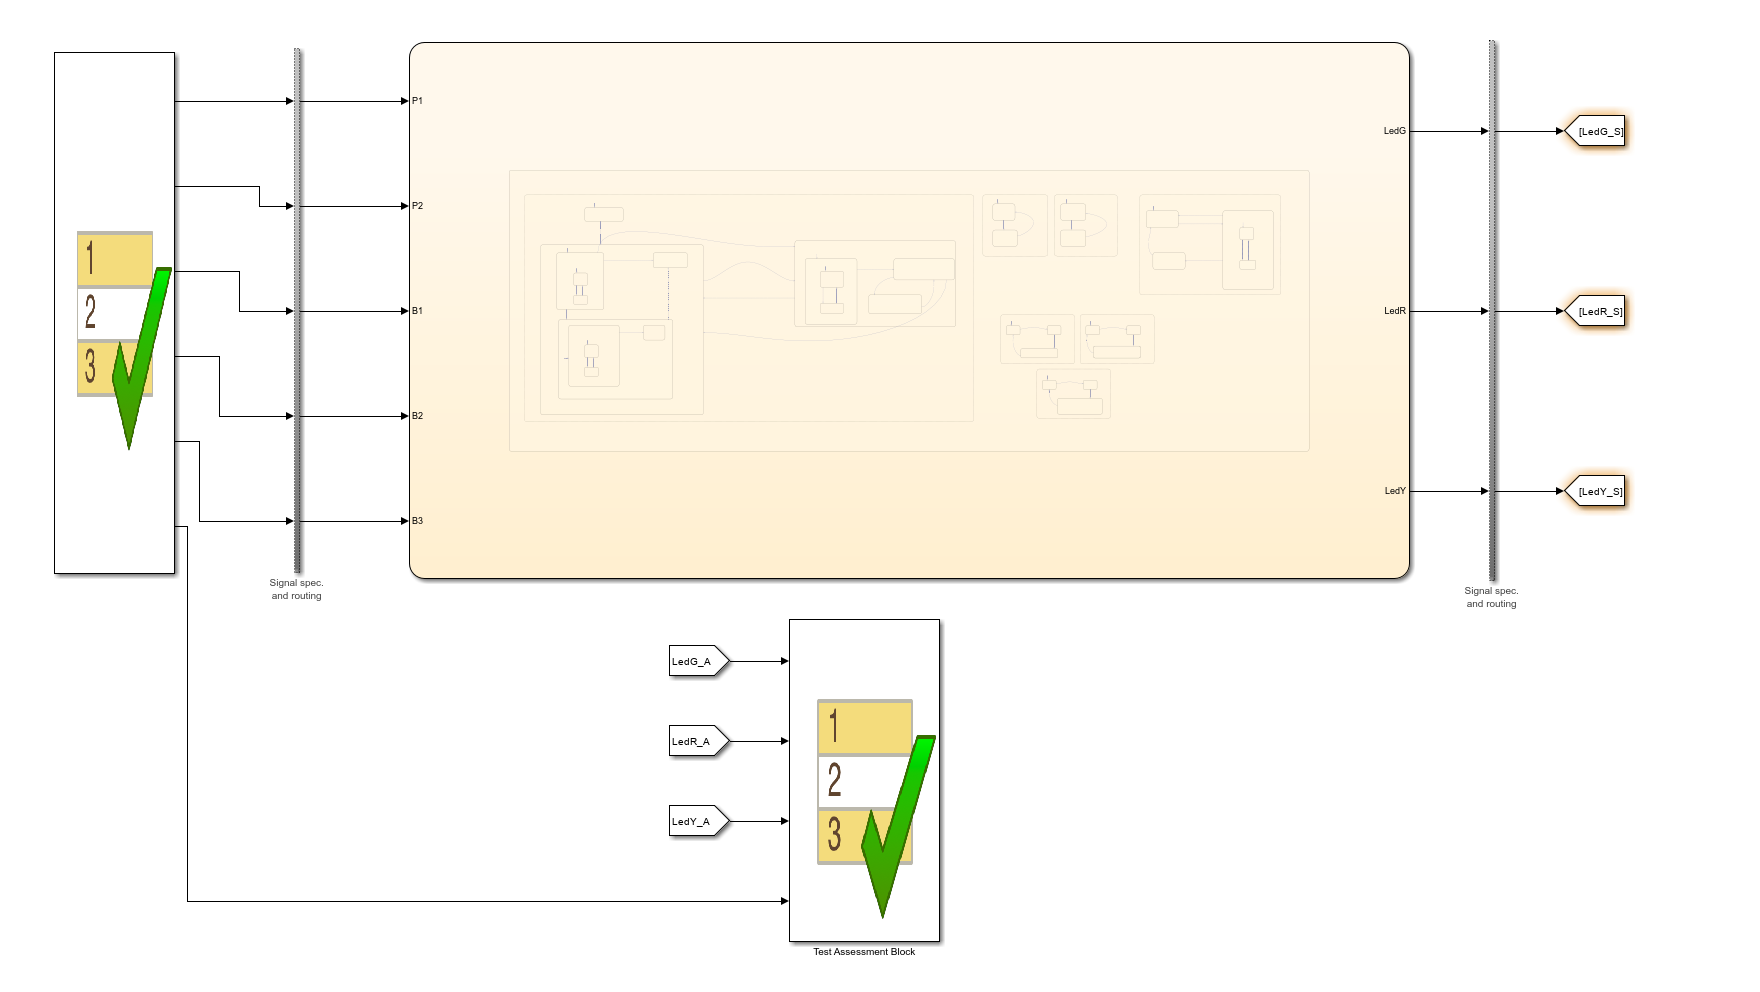
\includegraphics[width=0.6\textwidth]{figures/testharness.png}
        \caption{Esempio Test Harness}
        \label{harness}
    \end{figure}


    \section{Test Apertura e Chiusura Cancello}
        Di seguito è riportato il test relativo alla verifica della corretta apertura e chiusura del cancello quando l'utente preme il pulsante B1. In particolare, si effettua la verifica del corretto lampeggio del LED giallo in fase di verifica, della totale accensione di tutti i LED in fase di apertura e del totale spegnimento di questi ultimi in fase di chiusura.

        \begin{figure}[H]
            \centering
            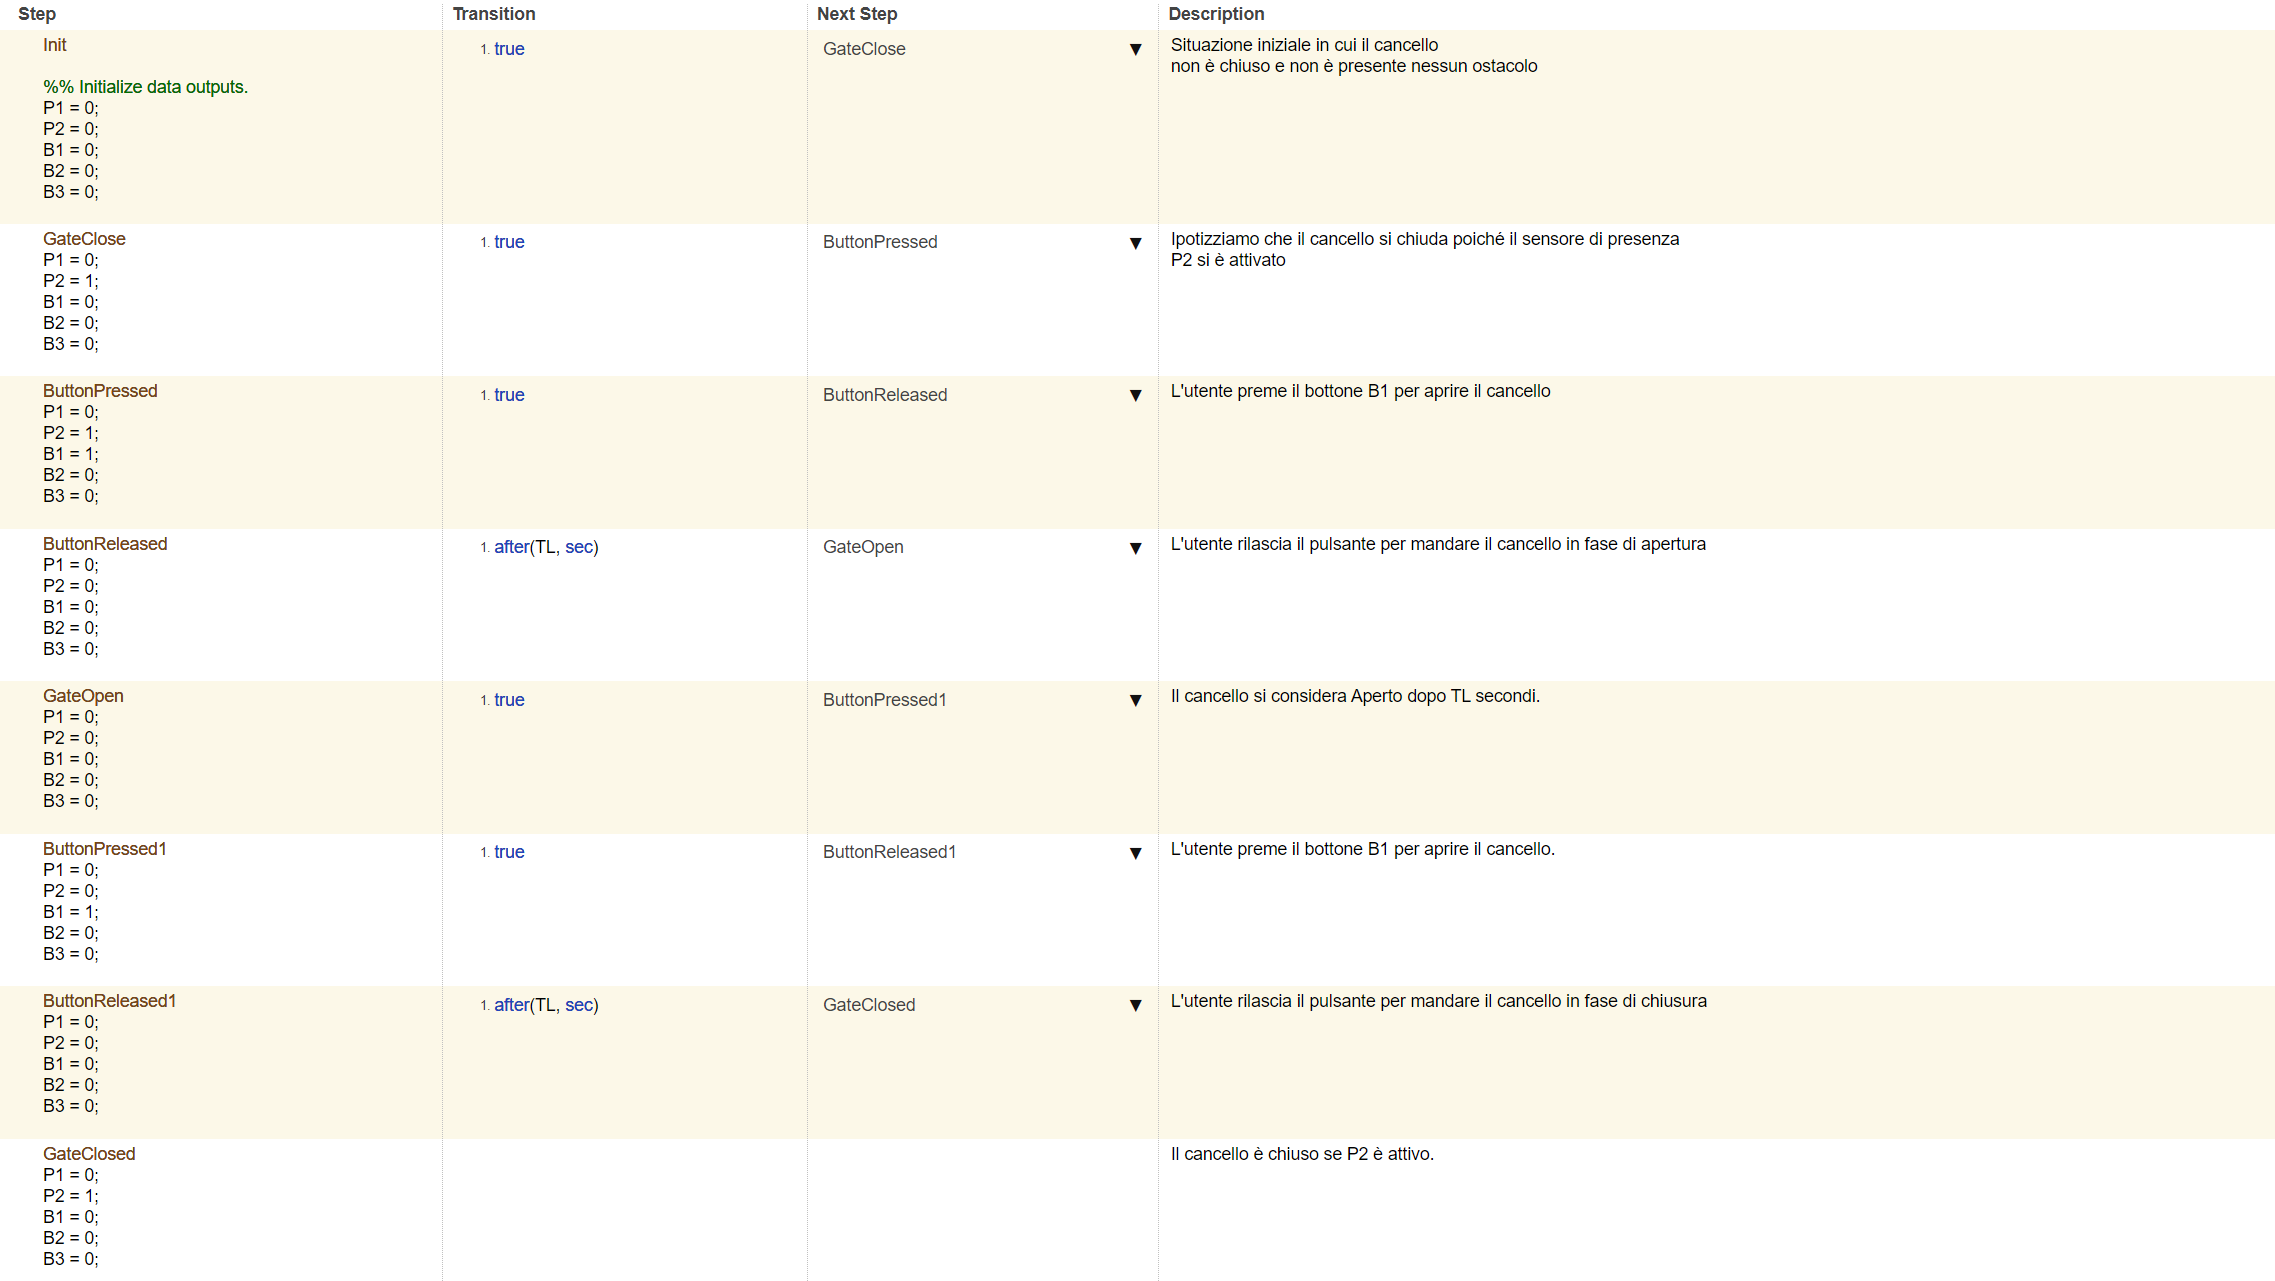
\includegraphics[width=0.9\textwidth]{figures/open_close.png}
            \caption{Test Sequence}
            \label{openclose}
        \end{figure}
    
        \begin{figure}[H]
            \centering
            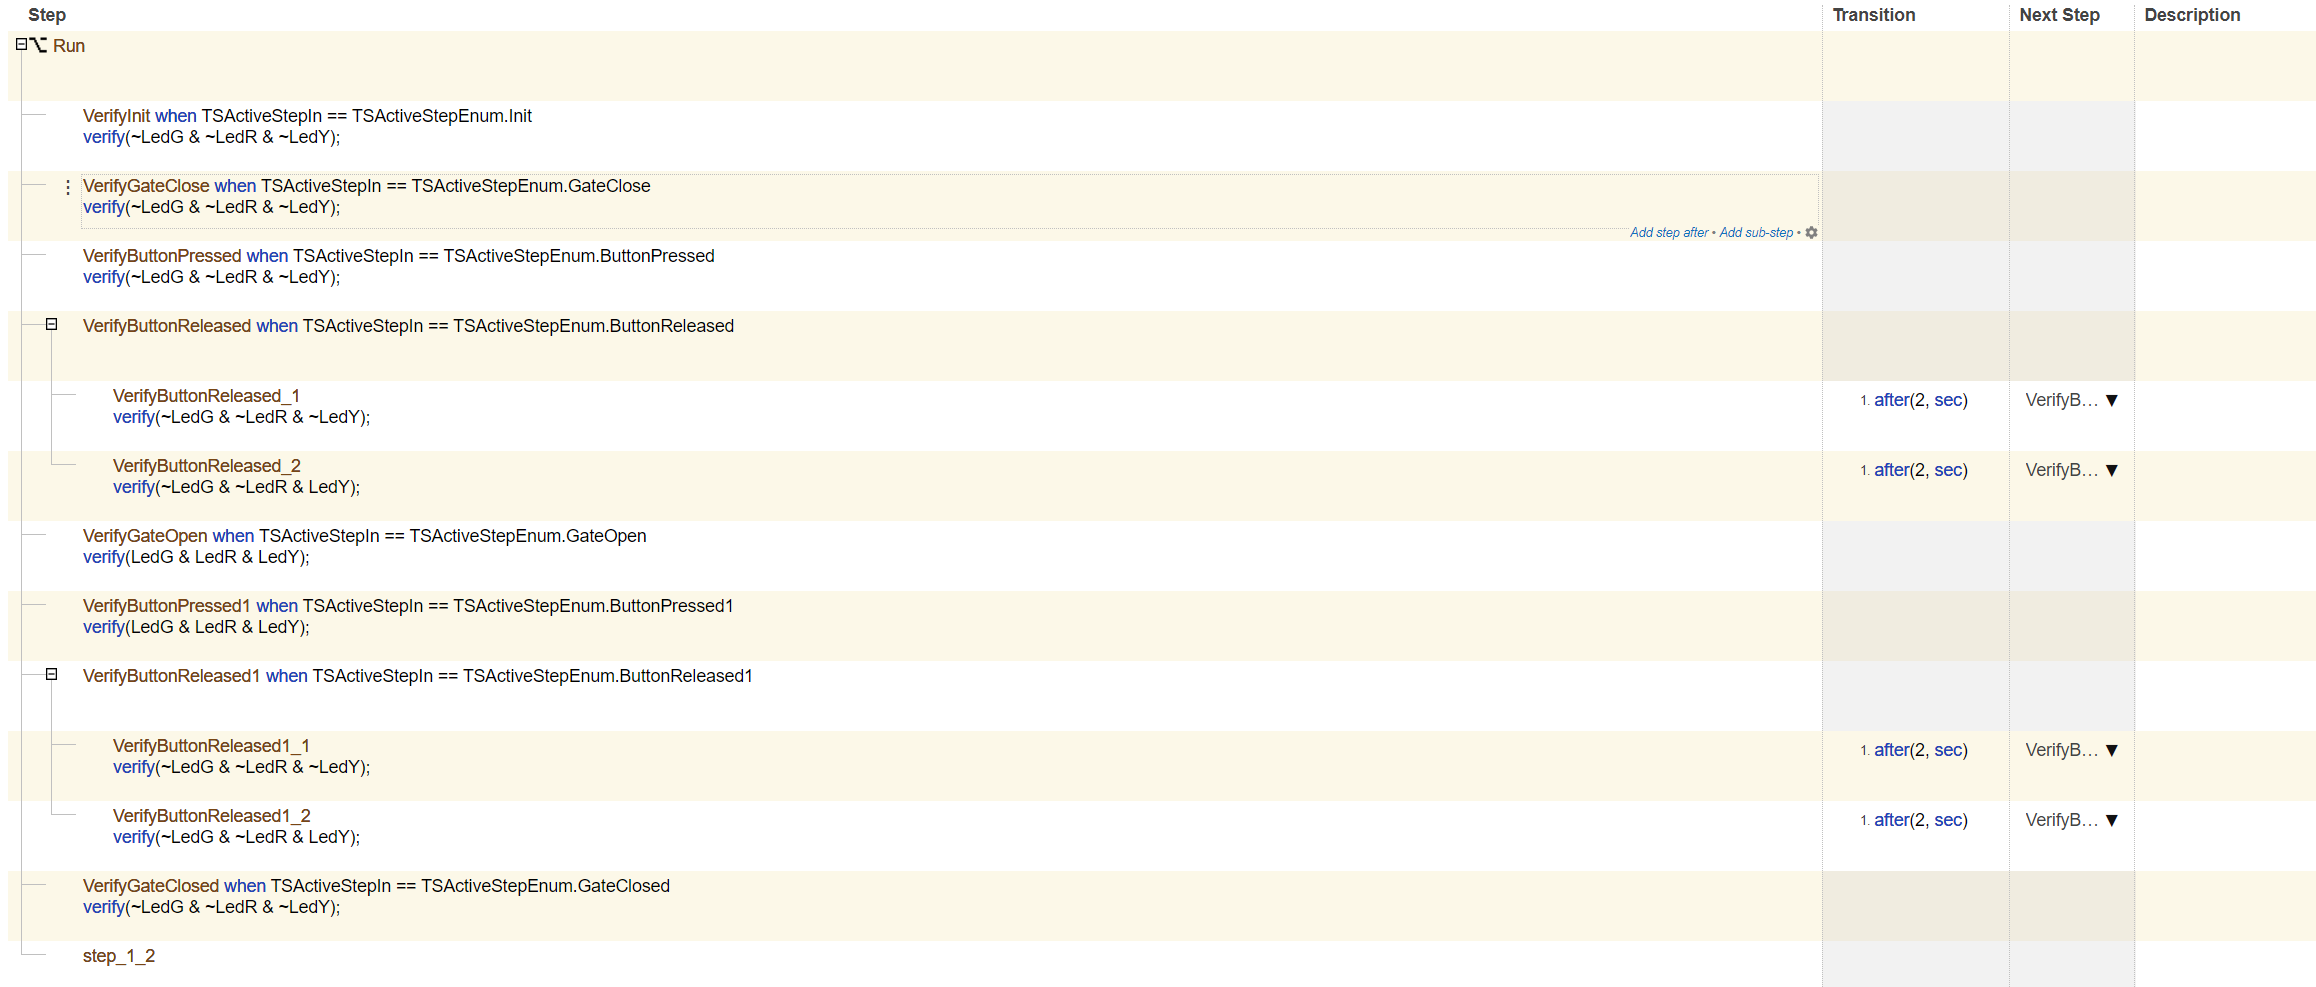
\includegraphics[width=0.9\textwidth]{figures/open_close2.png}
            \caption{Test Assessment}
            \label{openclose2}
        \end{figure}


    \section{Test Errore Cancello}
        Si riporta il test relativo alla verifica dello stato di errore del cancello qualora il sensore di presenza P2 non si attivi dopo $T_L$ secondi durante la fase di chiusura.
        Si ricorda che, dopo aver atteso tale tempo, il dispositivo attende ulteriori 10 secondi prima di accendere il LED rosso e segnalare la definitiva permanenza nello stato di errore.

        \begin{figure}[H]
            \centering
            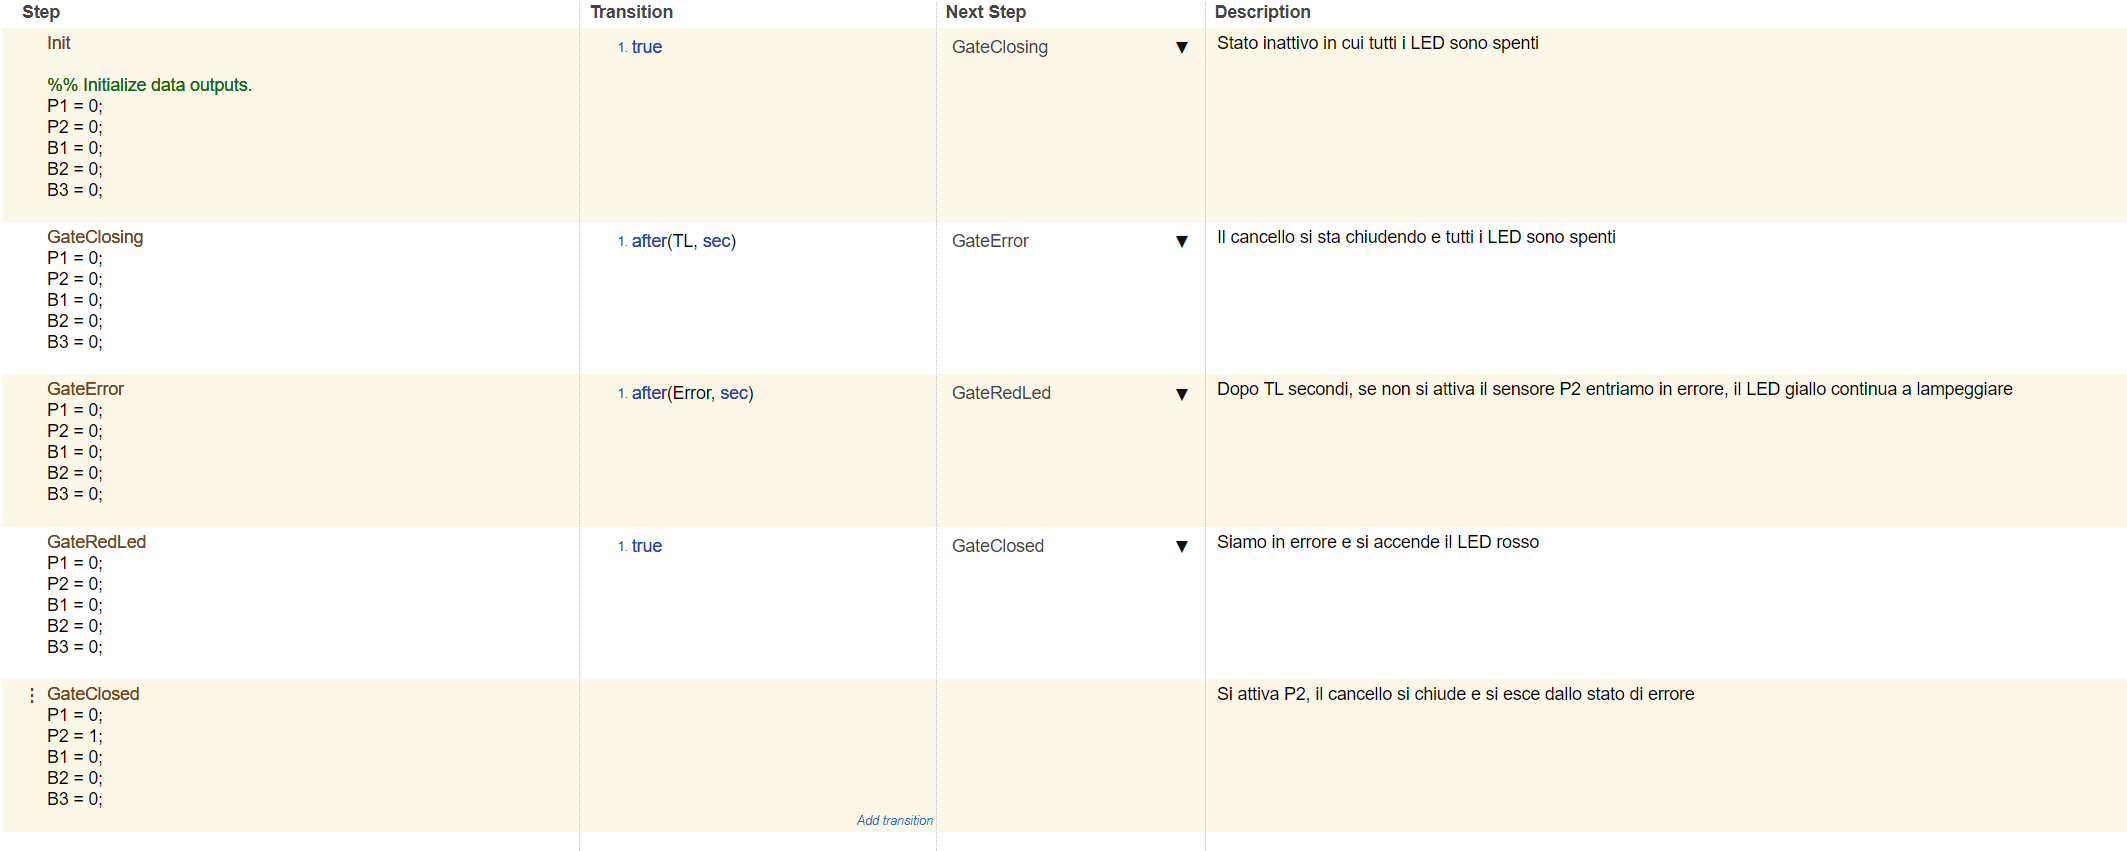
\includegraphics[width=0.9\textwidth]{figures/error.png}
            \caption{Test Sequence}
            \label{error}
        \end{figure}
    
        \begin{figure}[H]
            \centering
            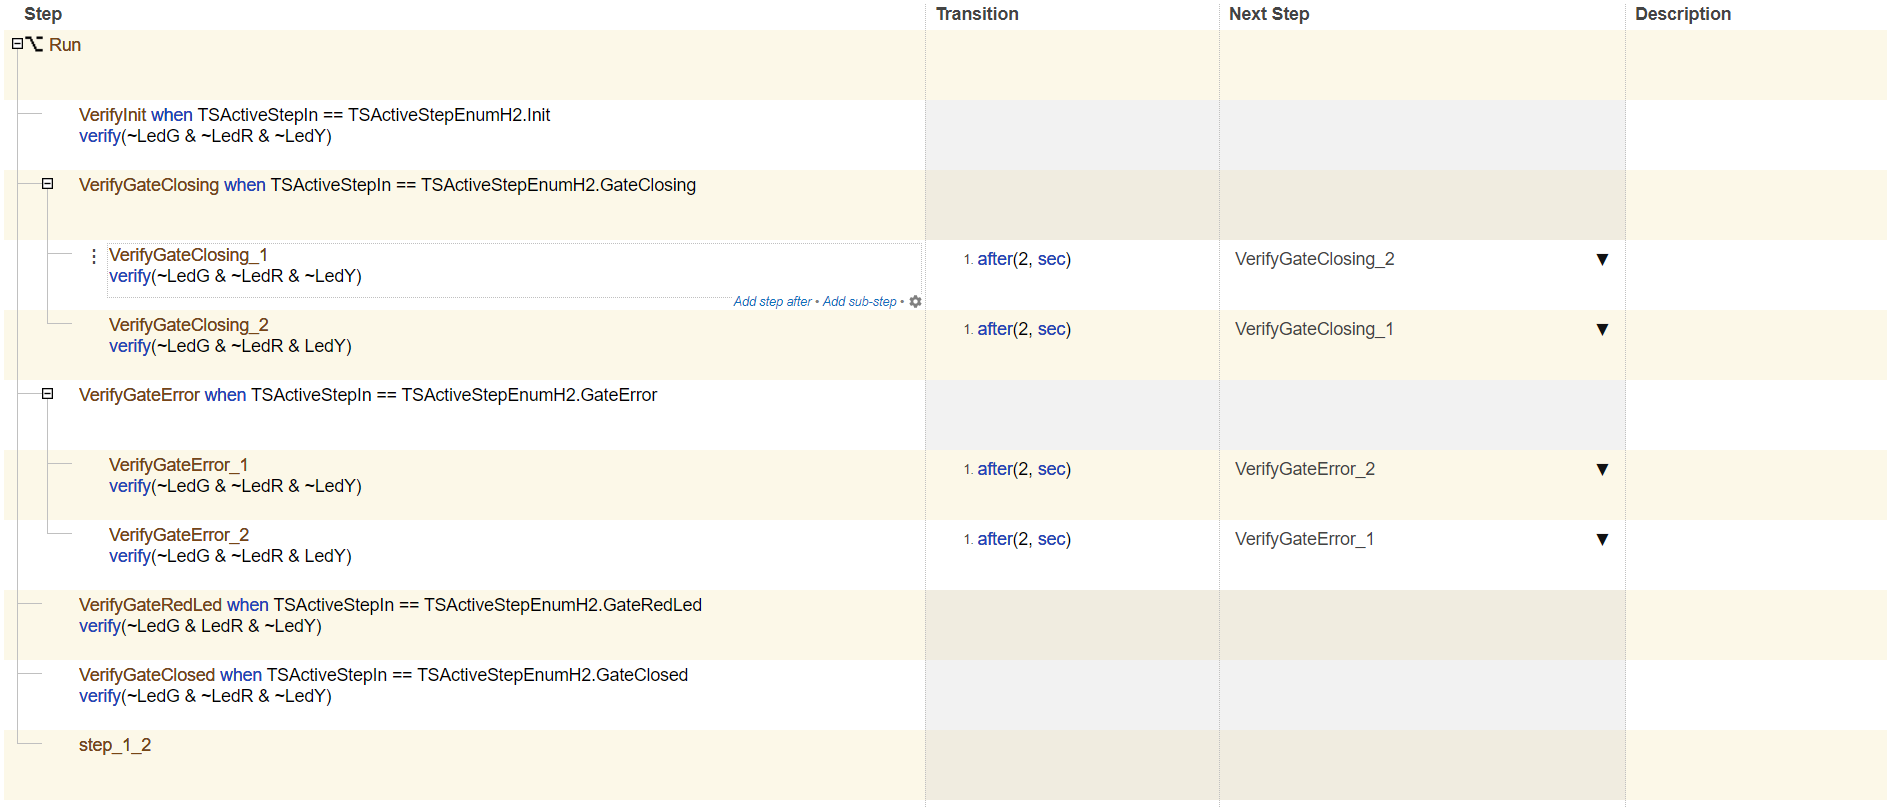
\includegraphics[width=0.9\textwidth]{figures/error2.png}
            \caption{Test Assessment}
            \label{error2}
        \end{figure}


    \section{Test Rilevazione Ostacolo se Aperto}
        Si riporta il test relativo alla rilevazione di un ostacolo quando il cancello si trova nello stato \textbf{Aperto}. Si ricorda che in caso di rilevazione positiva, mentre il cancello si sposta nello stato \textbf{Aperto con Ostacolo}, il macrostato \textbf{Ostacolo} permette il lampeggio del LED verde per un periodo di 30 secondi se l'utente tenta di chiudere il cancello con il sensore P1 attivo. 

        \begin{figure}[H]
            \centering
            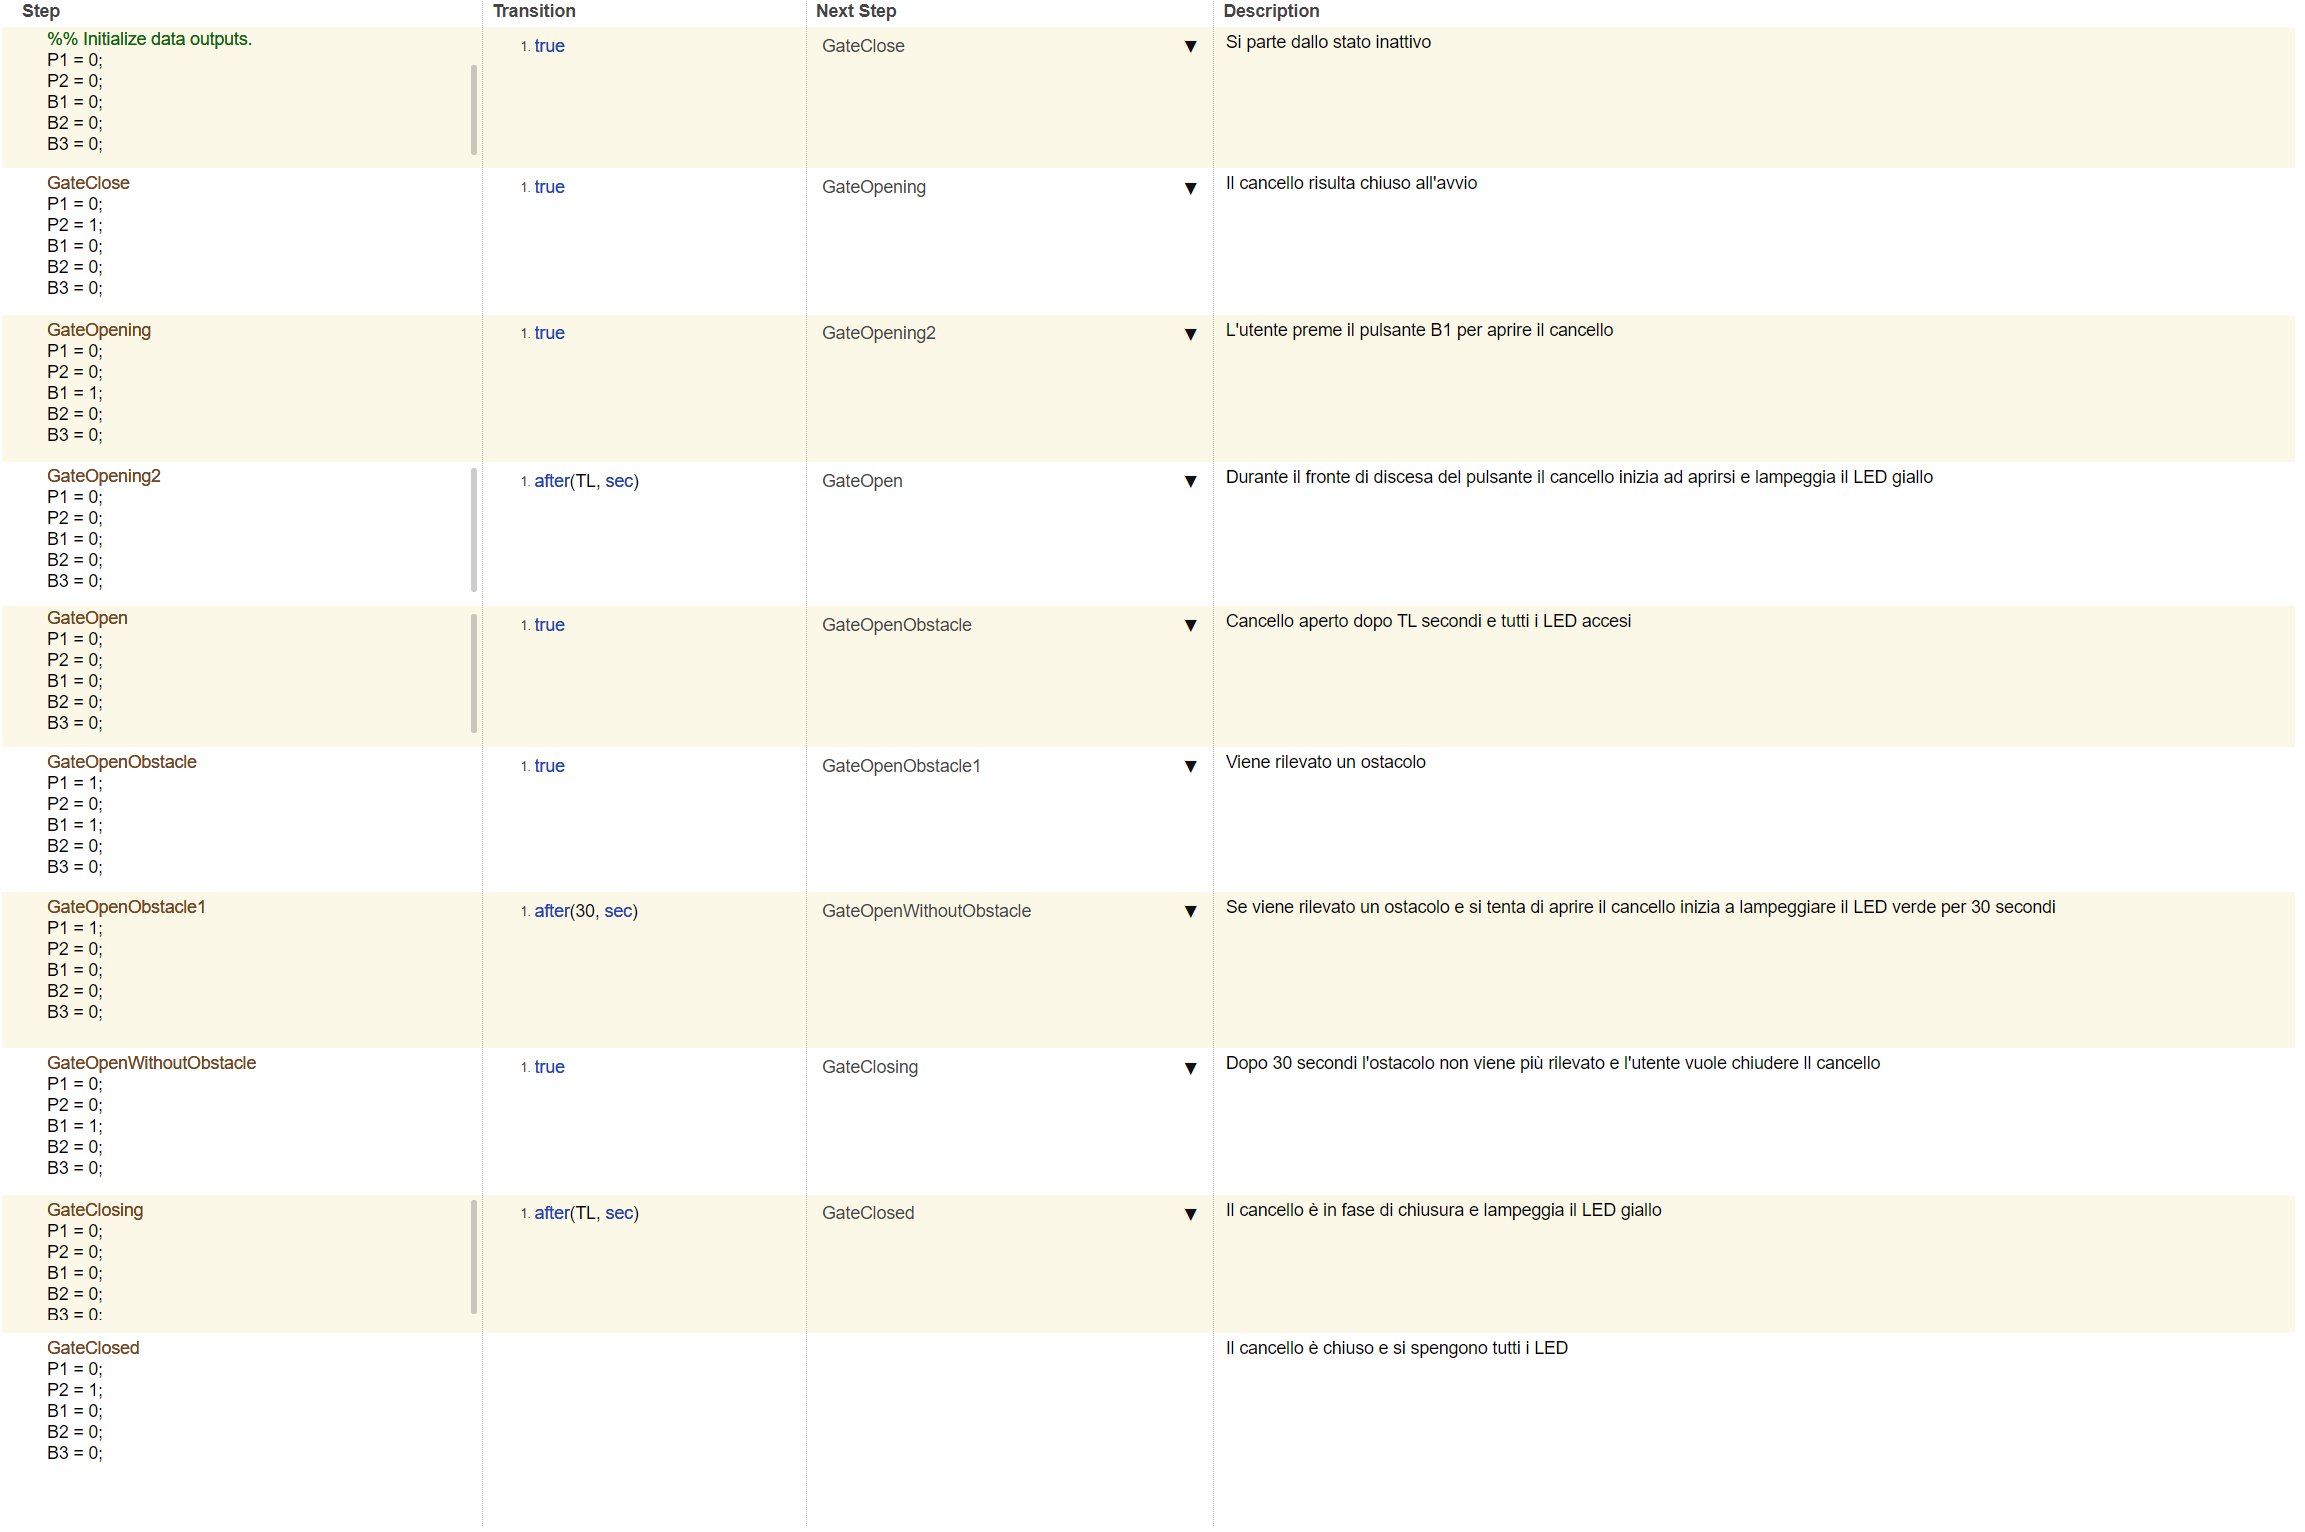
\includegraphics[width=0.9\textwidth]{figures/obstacletest.png}
            \caption{Test Sequence}
            \label{obtest}
        \end{figure}
    
        \begin{figure}[H]
            \centering
            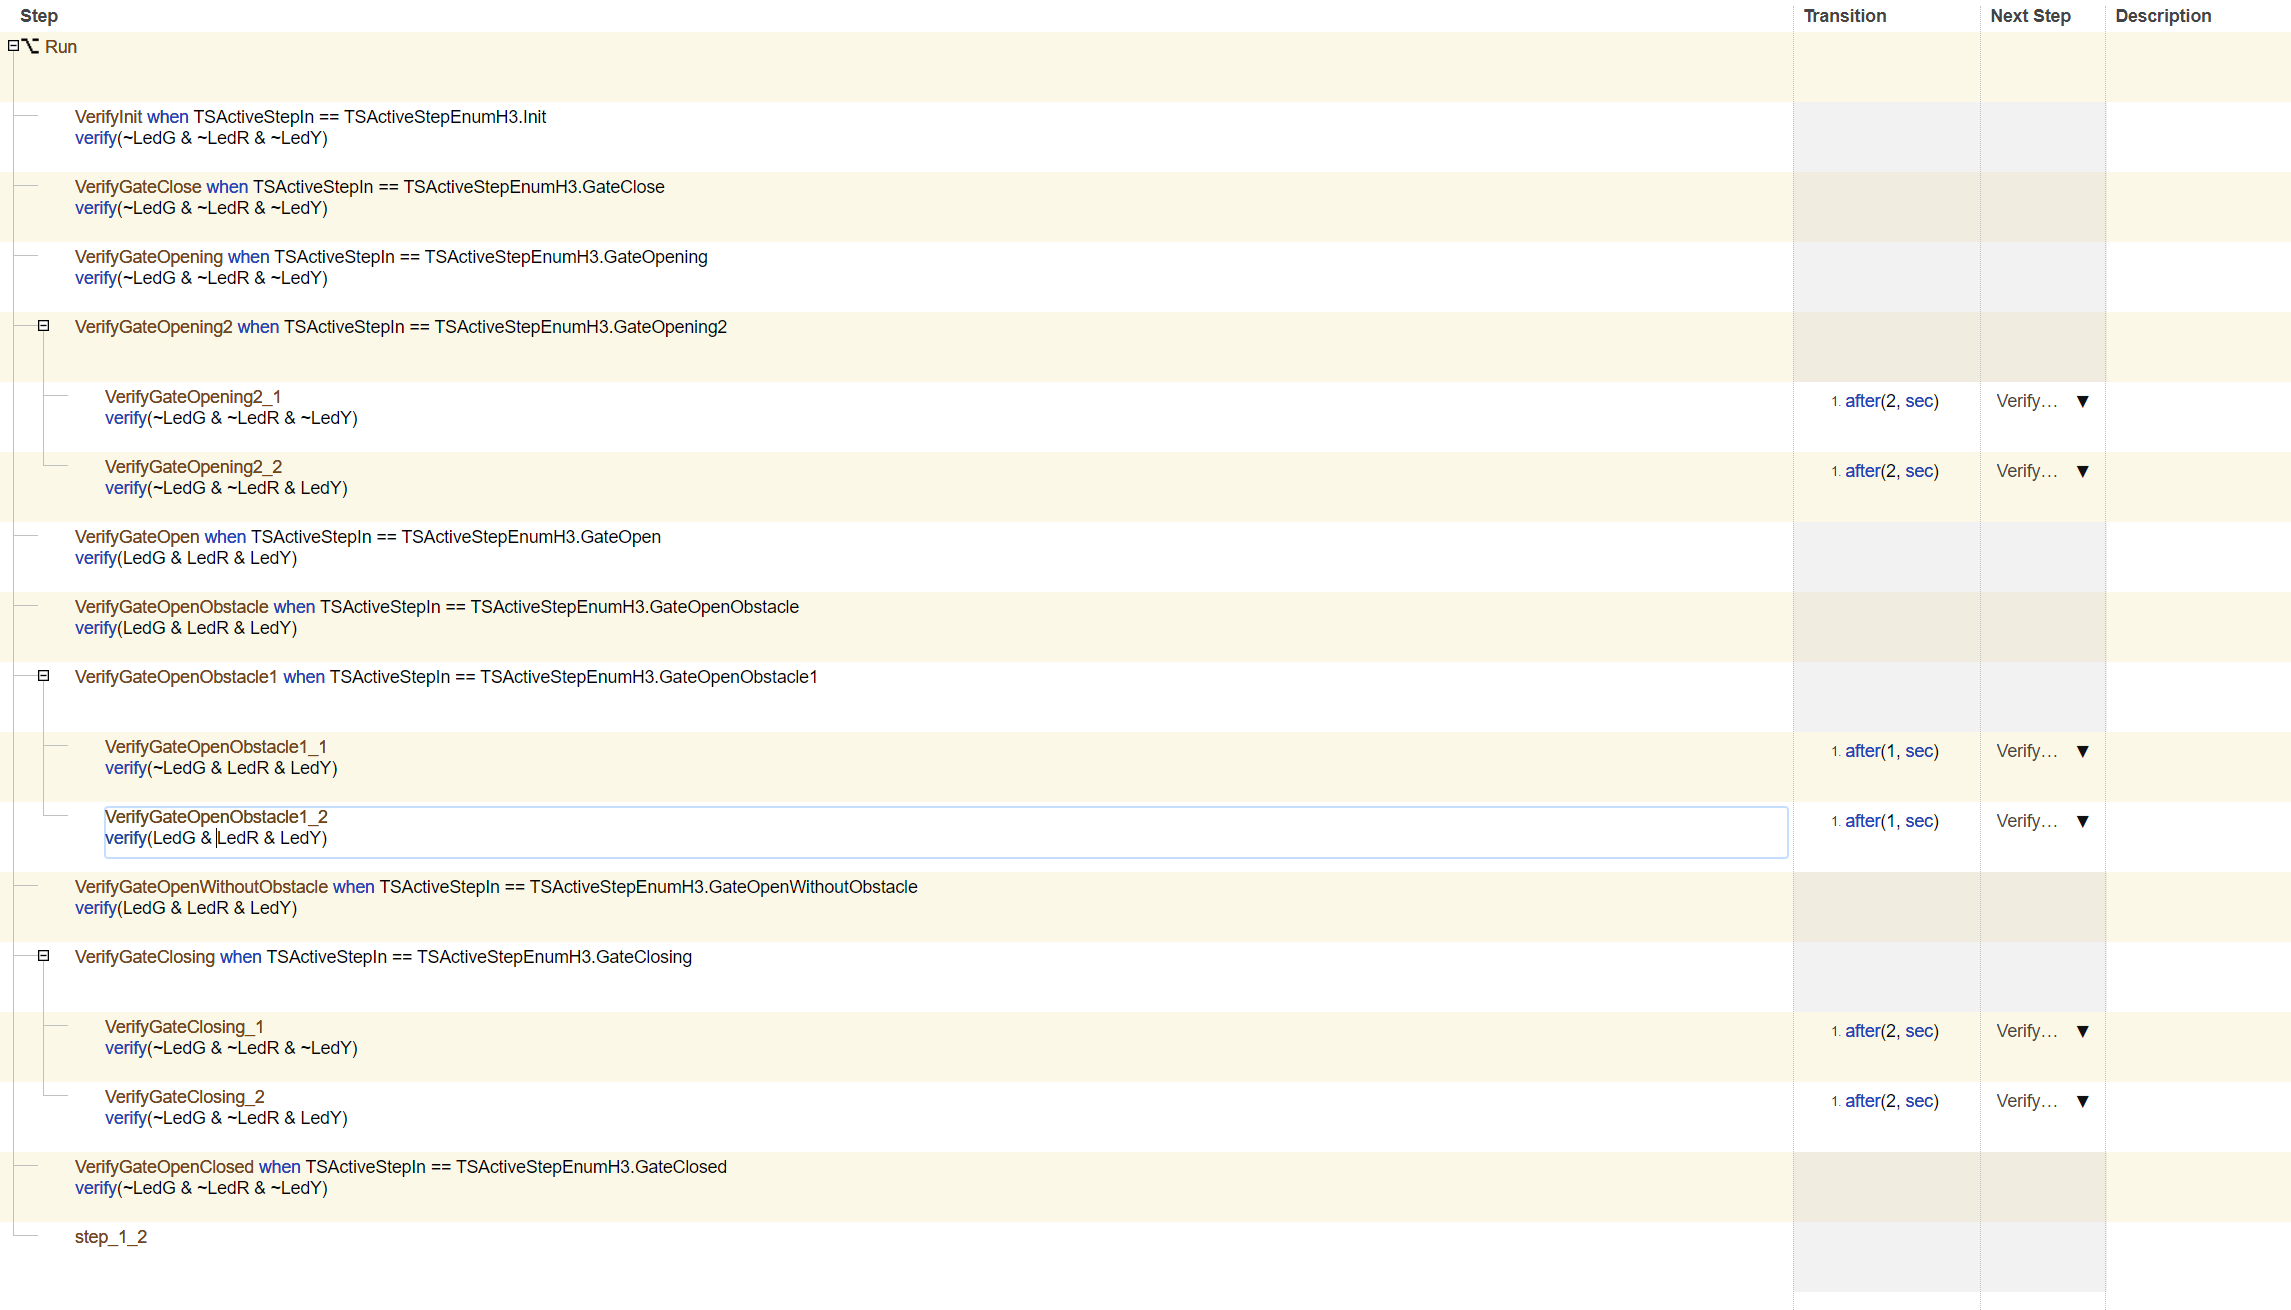
\includegraphics[width=0.9\textwidth]{figures/obstacletest1.png}
            \caption{Test Assessment}
            \label{obstest1}
        \end{figure}


    \section{Test Rilevazione Ostacolo se In Chiusura}
        Si riporta il test relativo alla rilevazione di un ostacolo quando il cancello è in fase di chiusura.
        In particolare, il cancello si sposta in fase di apertura continuando il lampeggio del LED giallo per poi aprirsi completamente.
        In seguito, il test prevede l'attesa del tempo di chiusura automatica $T_C$ per poi chiudersi definitivamente.

        \begin{figure}[H]
            \centering
            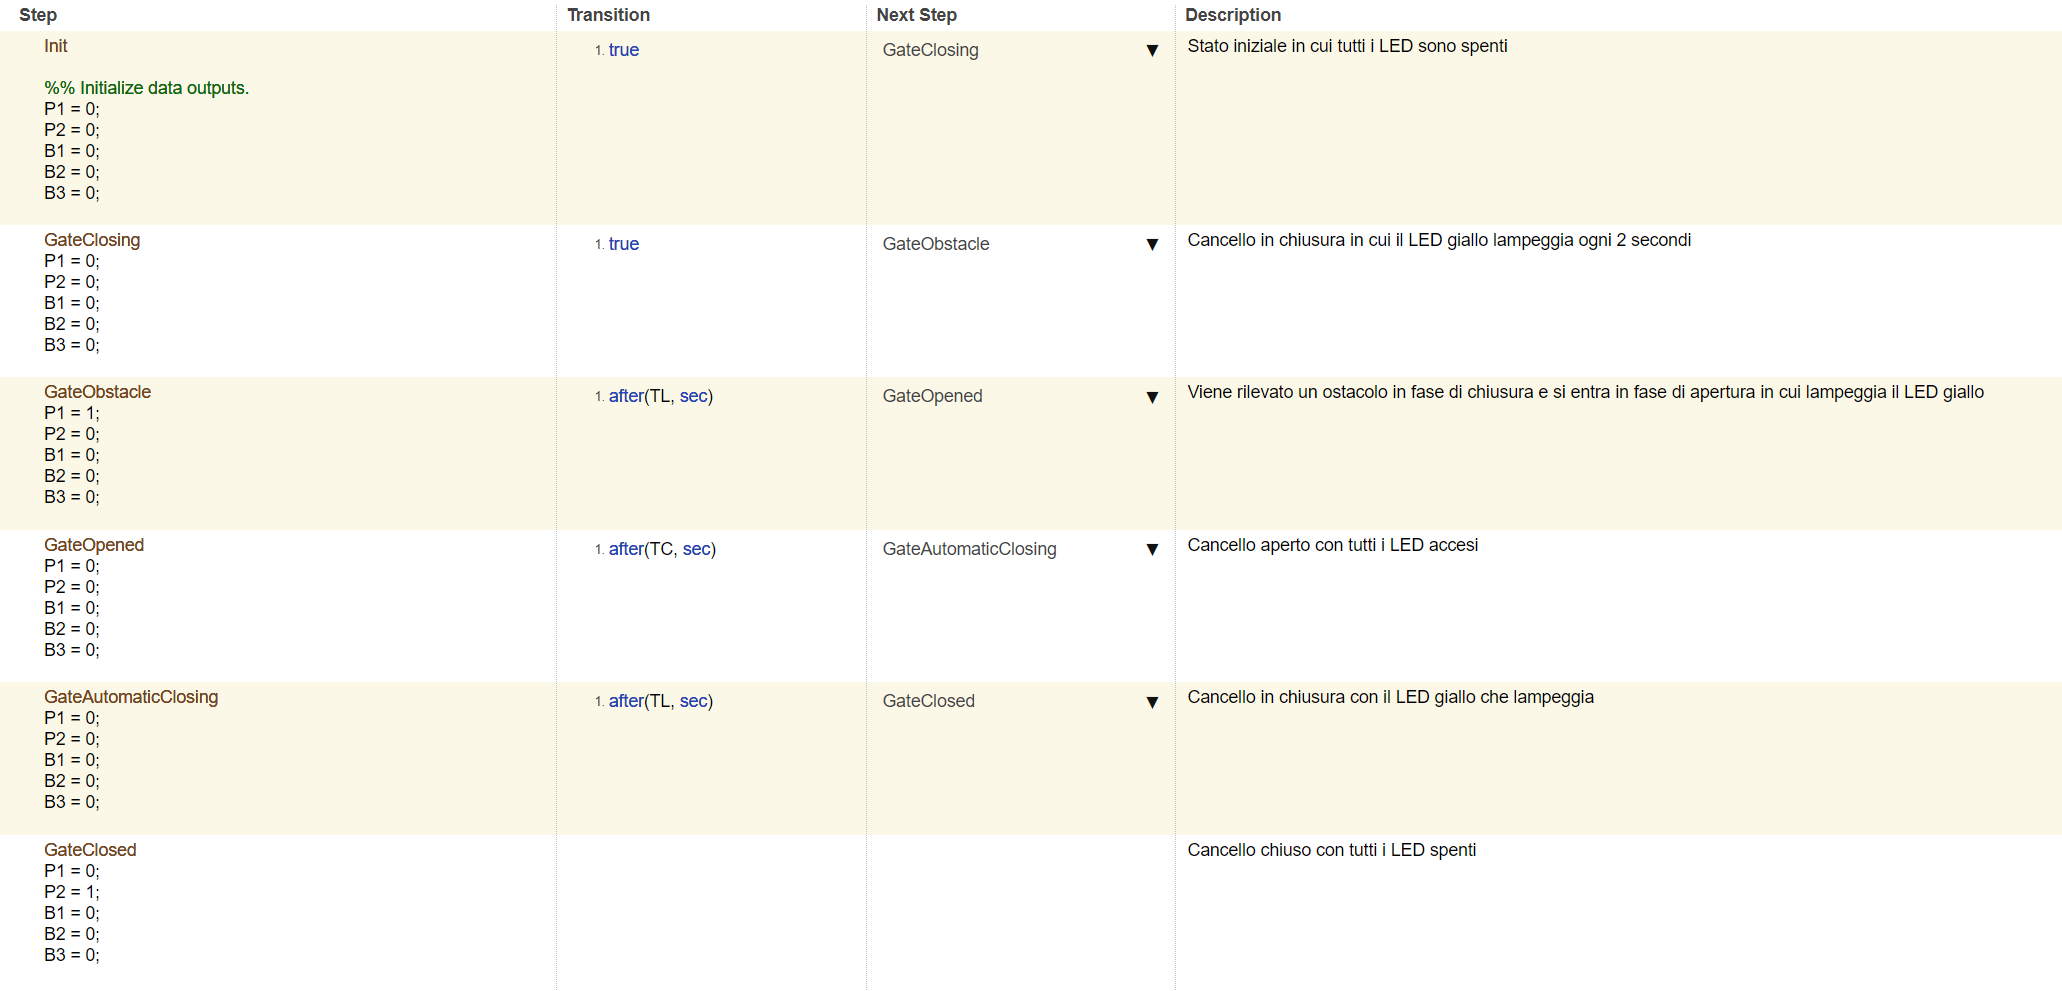
\includegraphics[width=0.9\textwidth]{figures/automaticclosing.png}
            \caption{Test Sequence}
            \label{autom}
        \end{figure}
        
        \begin{figure}[H]
            \centering
            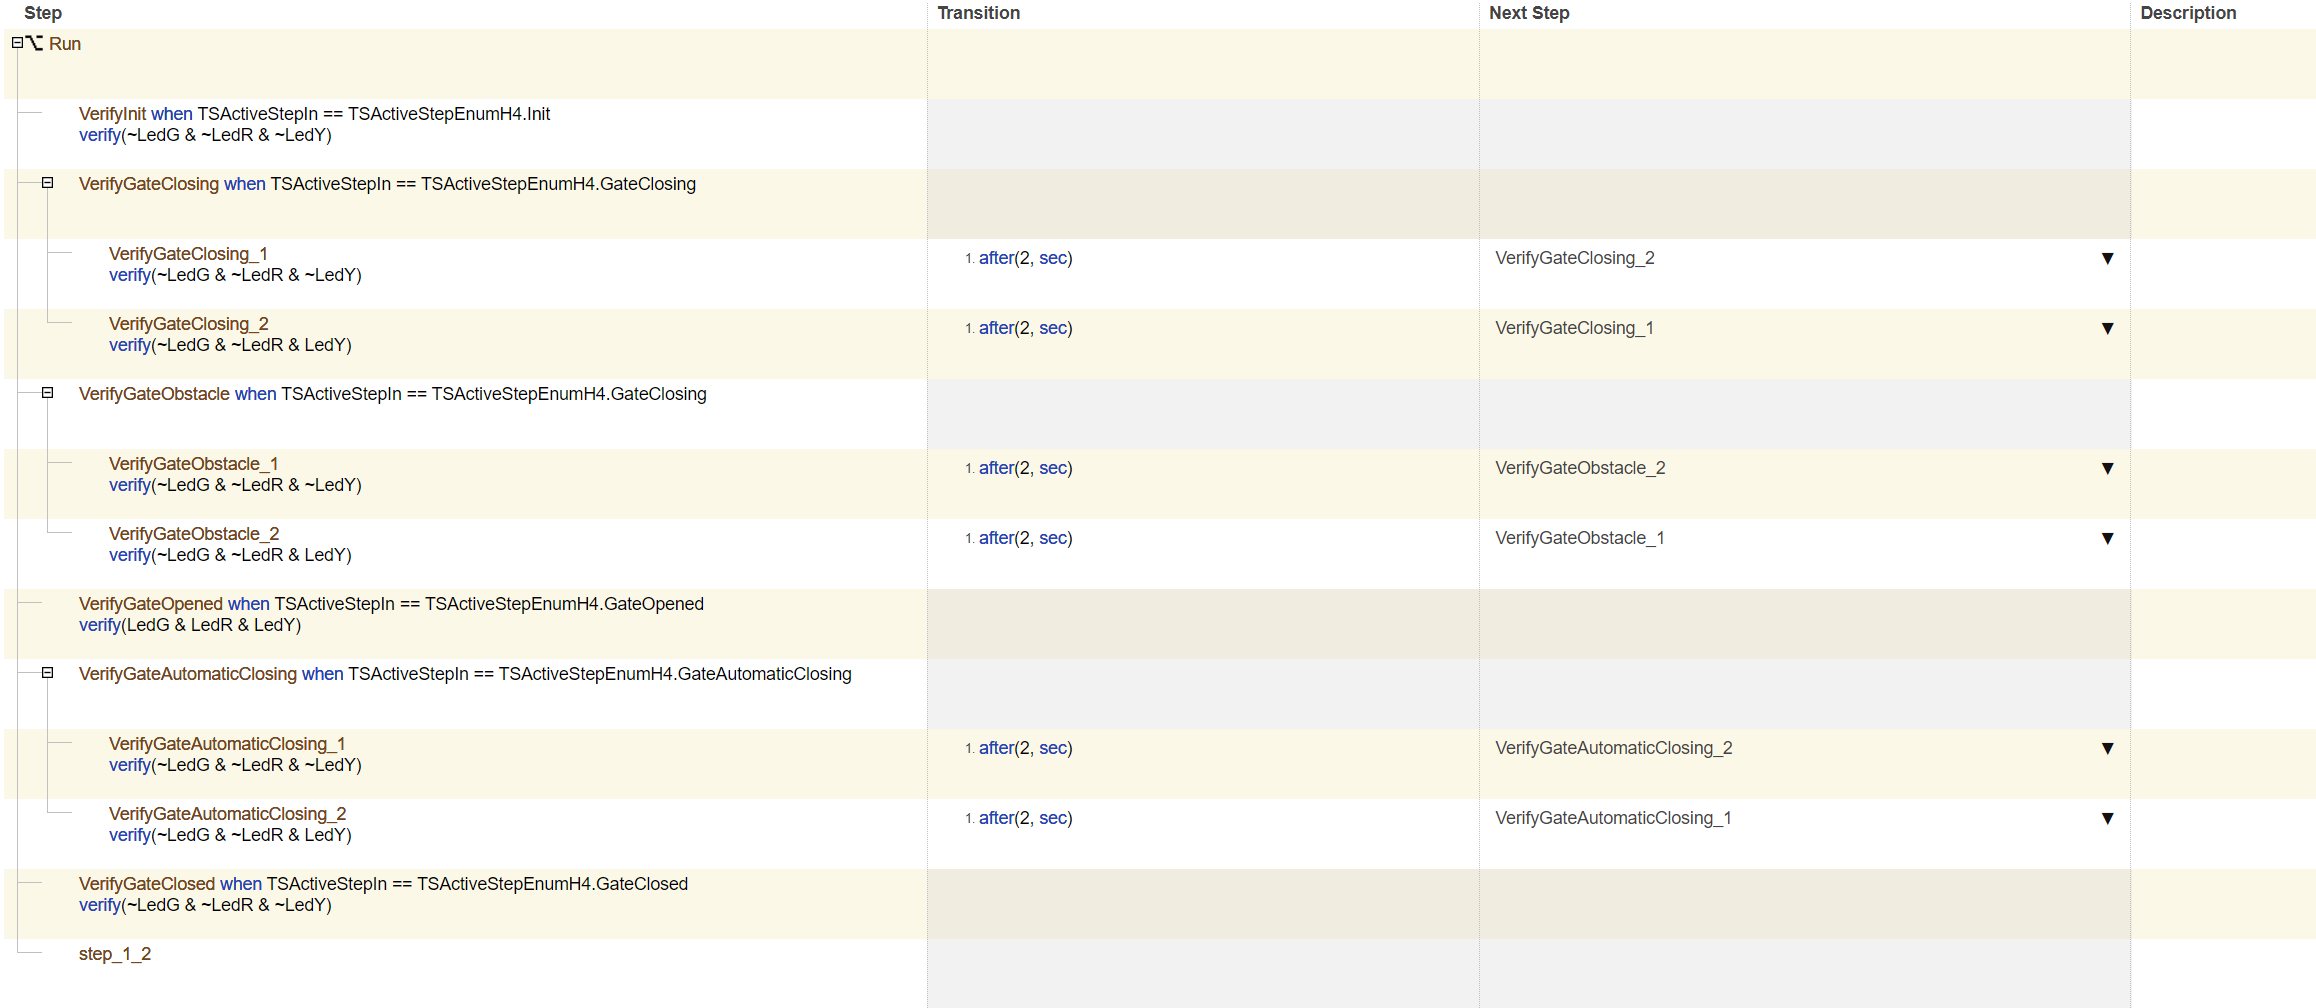
\includegraphics[width=0.9\textwidth]{figures/automaticclosing1.png}
            \caption{Test Assessment}
            \label{autom1}
        \end{figure}

    
    \section{Test Rilevazione Ostacolo se Chiuso}
        Si riporta il test relativo alla rilevazione di un ostacolo quando il cancello è chiuso. In particolare, il cancello non si apre se l'utente preme il pulsante B1, ma inizia il lampeggio del LED verde per 30 secondi, per poi spegnersi insieme agli altri due LED.

        \begin{figure}[H]
            \centering
            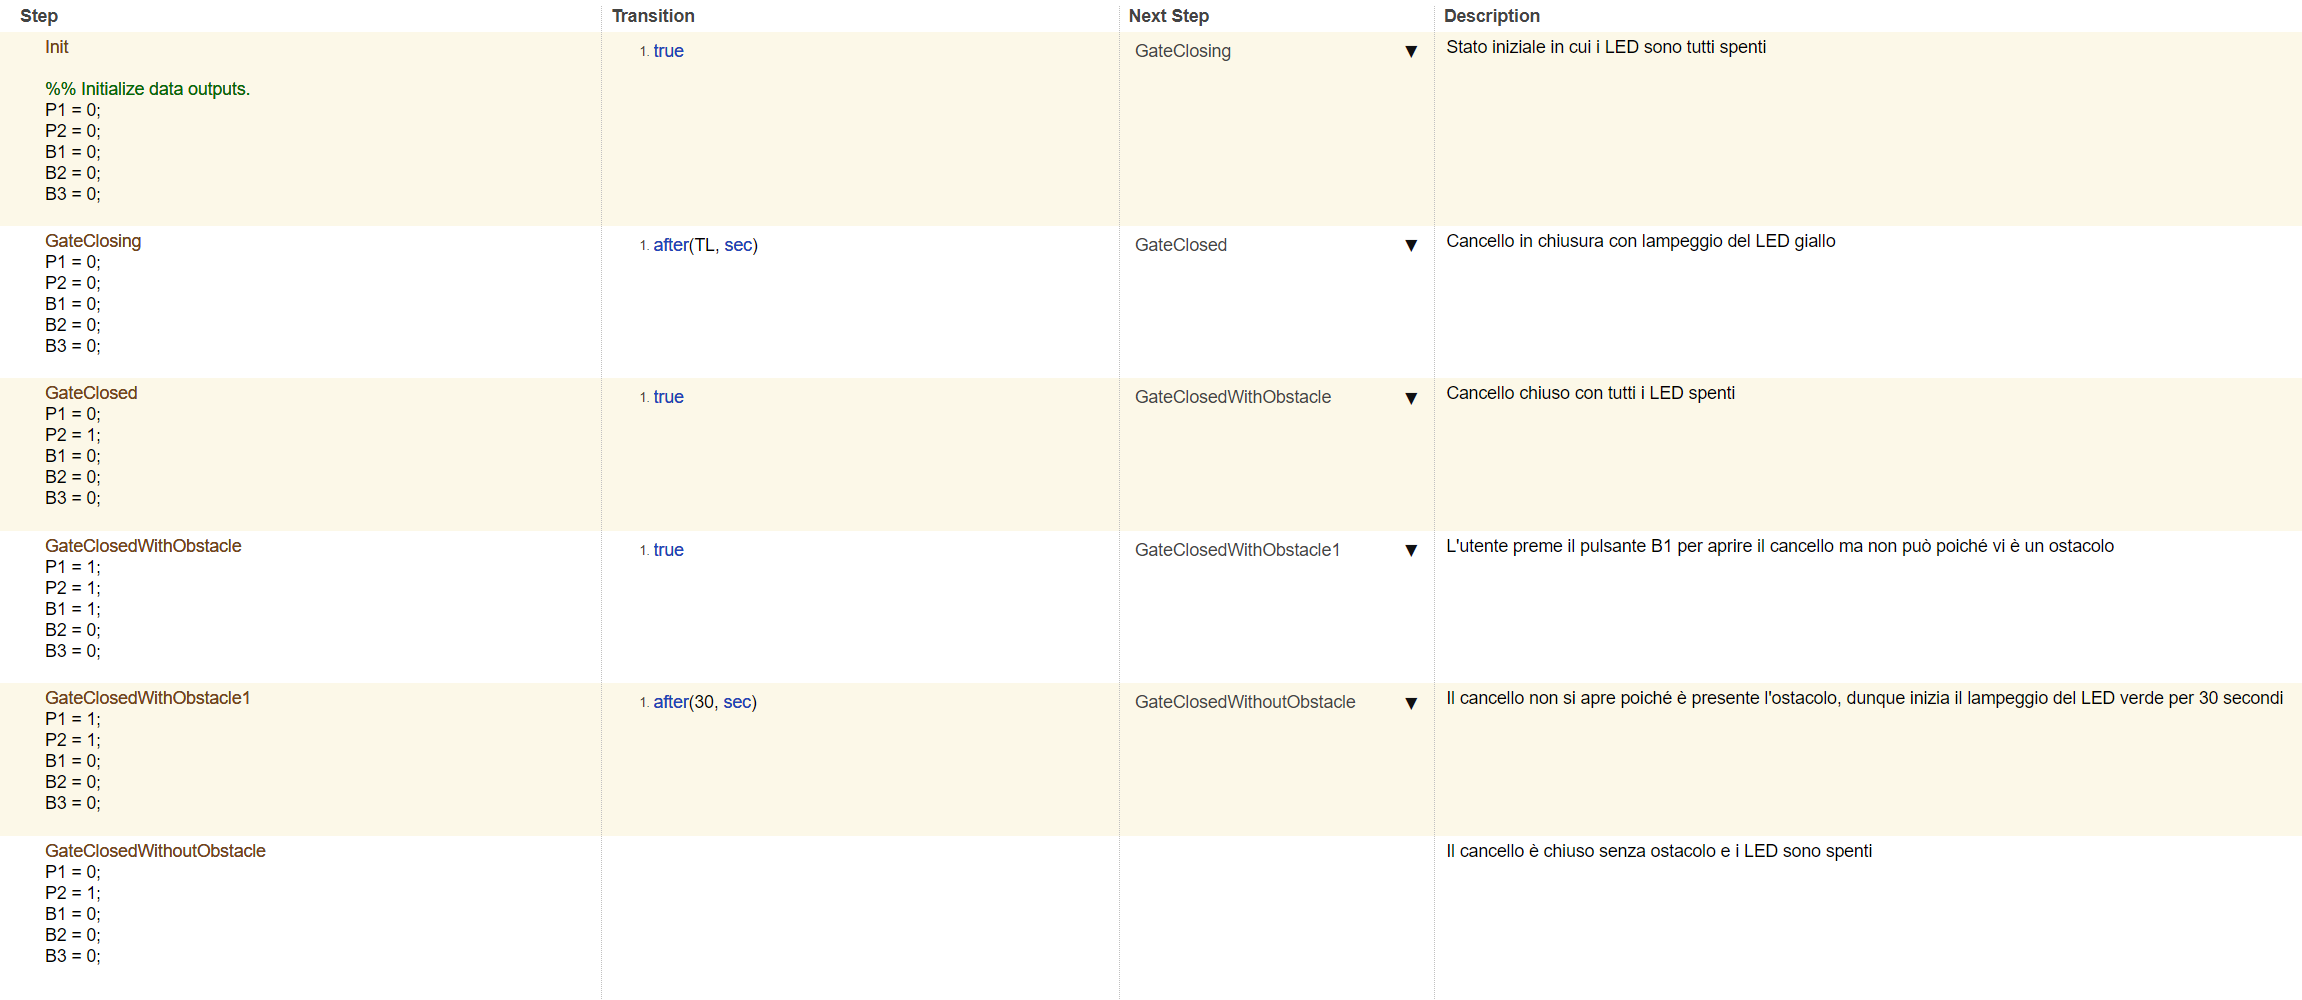
\includegraphics[width=0.9\textwidth]{figures/closedobs.png}
            \caption{Test Sequence}
            \label{closeobs}
        \end{figure}
        
        \begin{figure}[H]
            \centering
            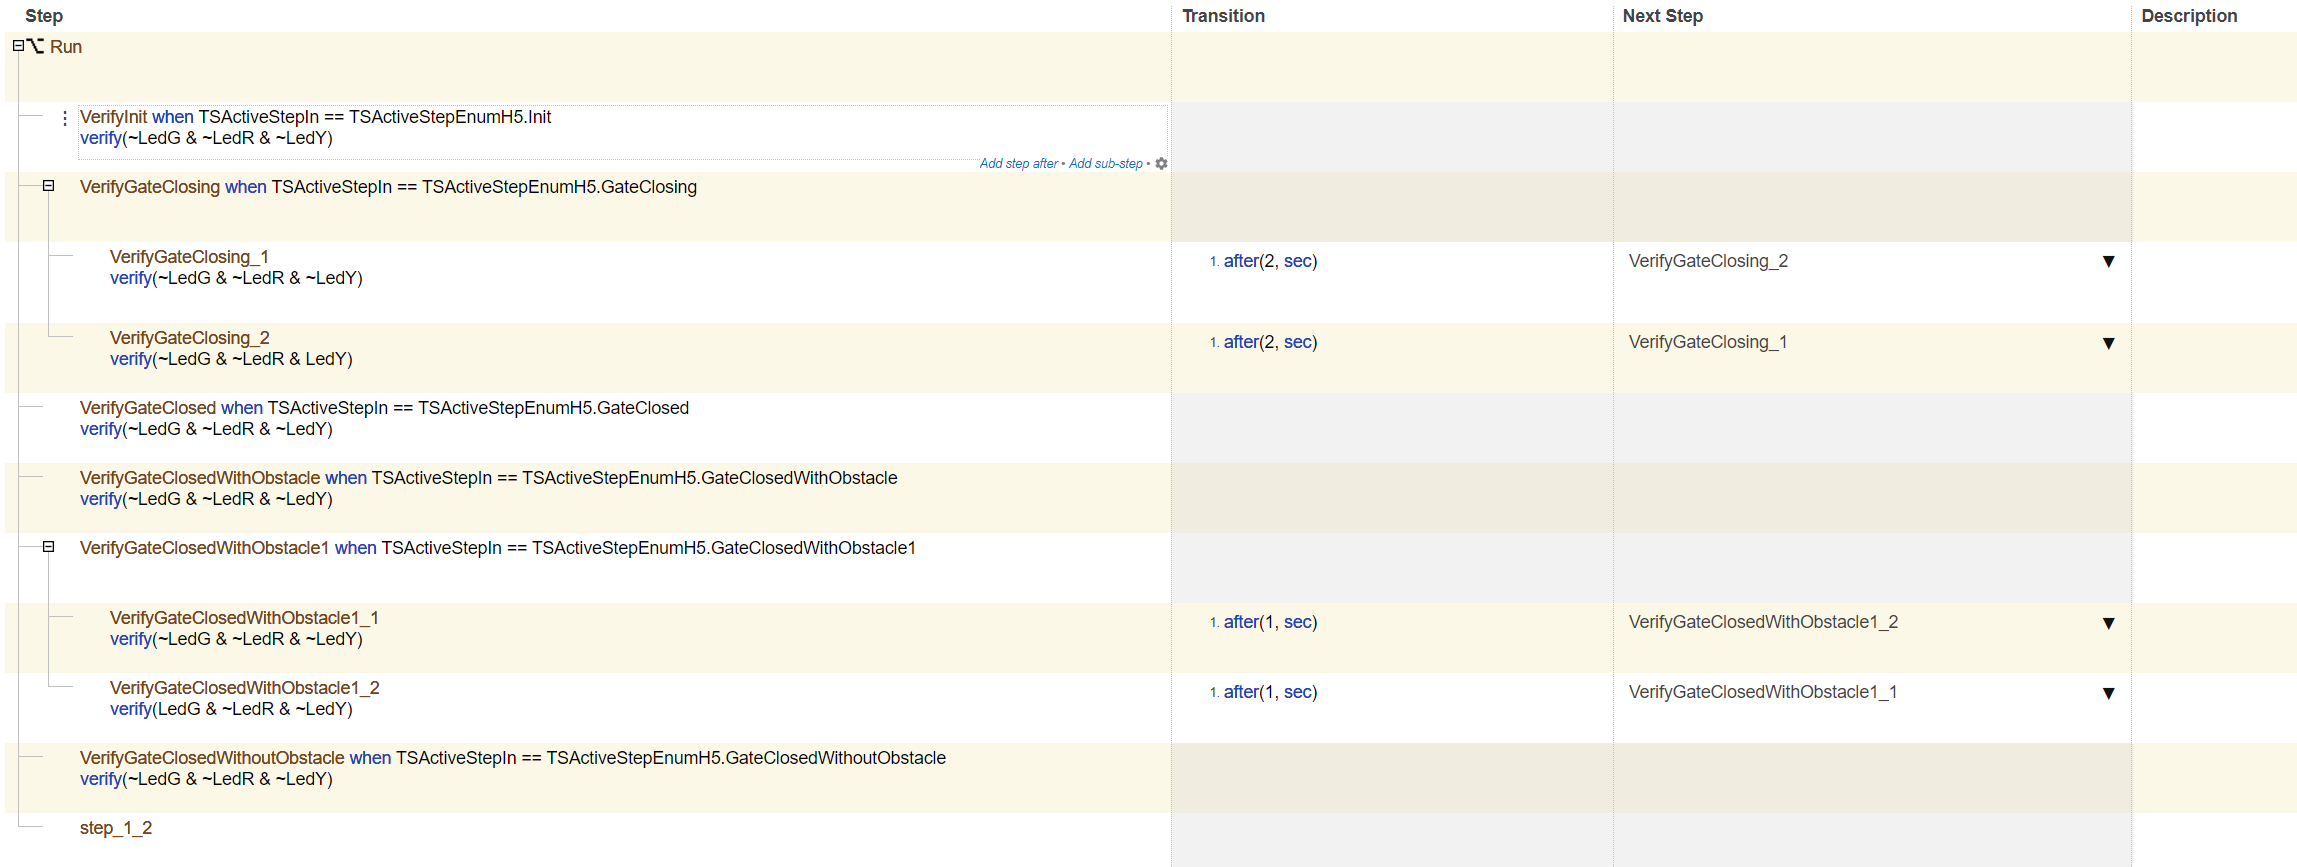
\includegraphics[width=0.9\textwidth]{figures/closedobs1.png}
            \caption{Test Assessment}
            \label{closeobs1}
        \end{figure}

    
    \section{Regolazione $T_C$ e $T_L$}
        Si riporta il test relativo alla regolazione del tempo di lavoro e del tempo di chiusura.
        In particolare, il cancello si chiude inizialmente con $T_L$ pari a 10 secondi.
        In seguito, l'utente preme il pulsante B2 e B3 per aumentare sia $T_L$ che $T_C$ di 10 secondi.
        Dopodiché, il cancello viene portato in fase di apertura (e successivamente chiusura) con il nuovo tempo di lavoro.

        \begin{figure}[H]
            \centering
            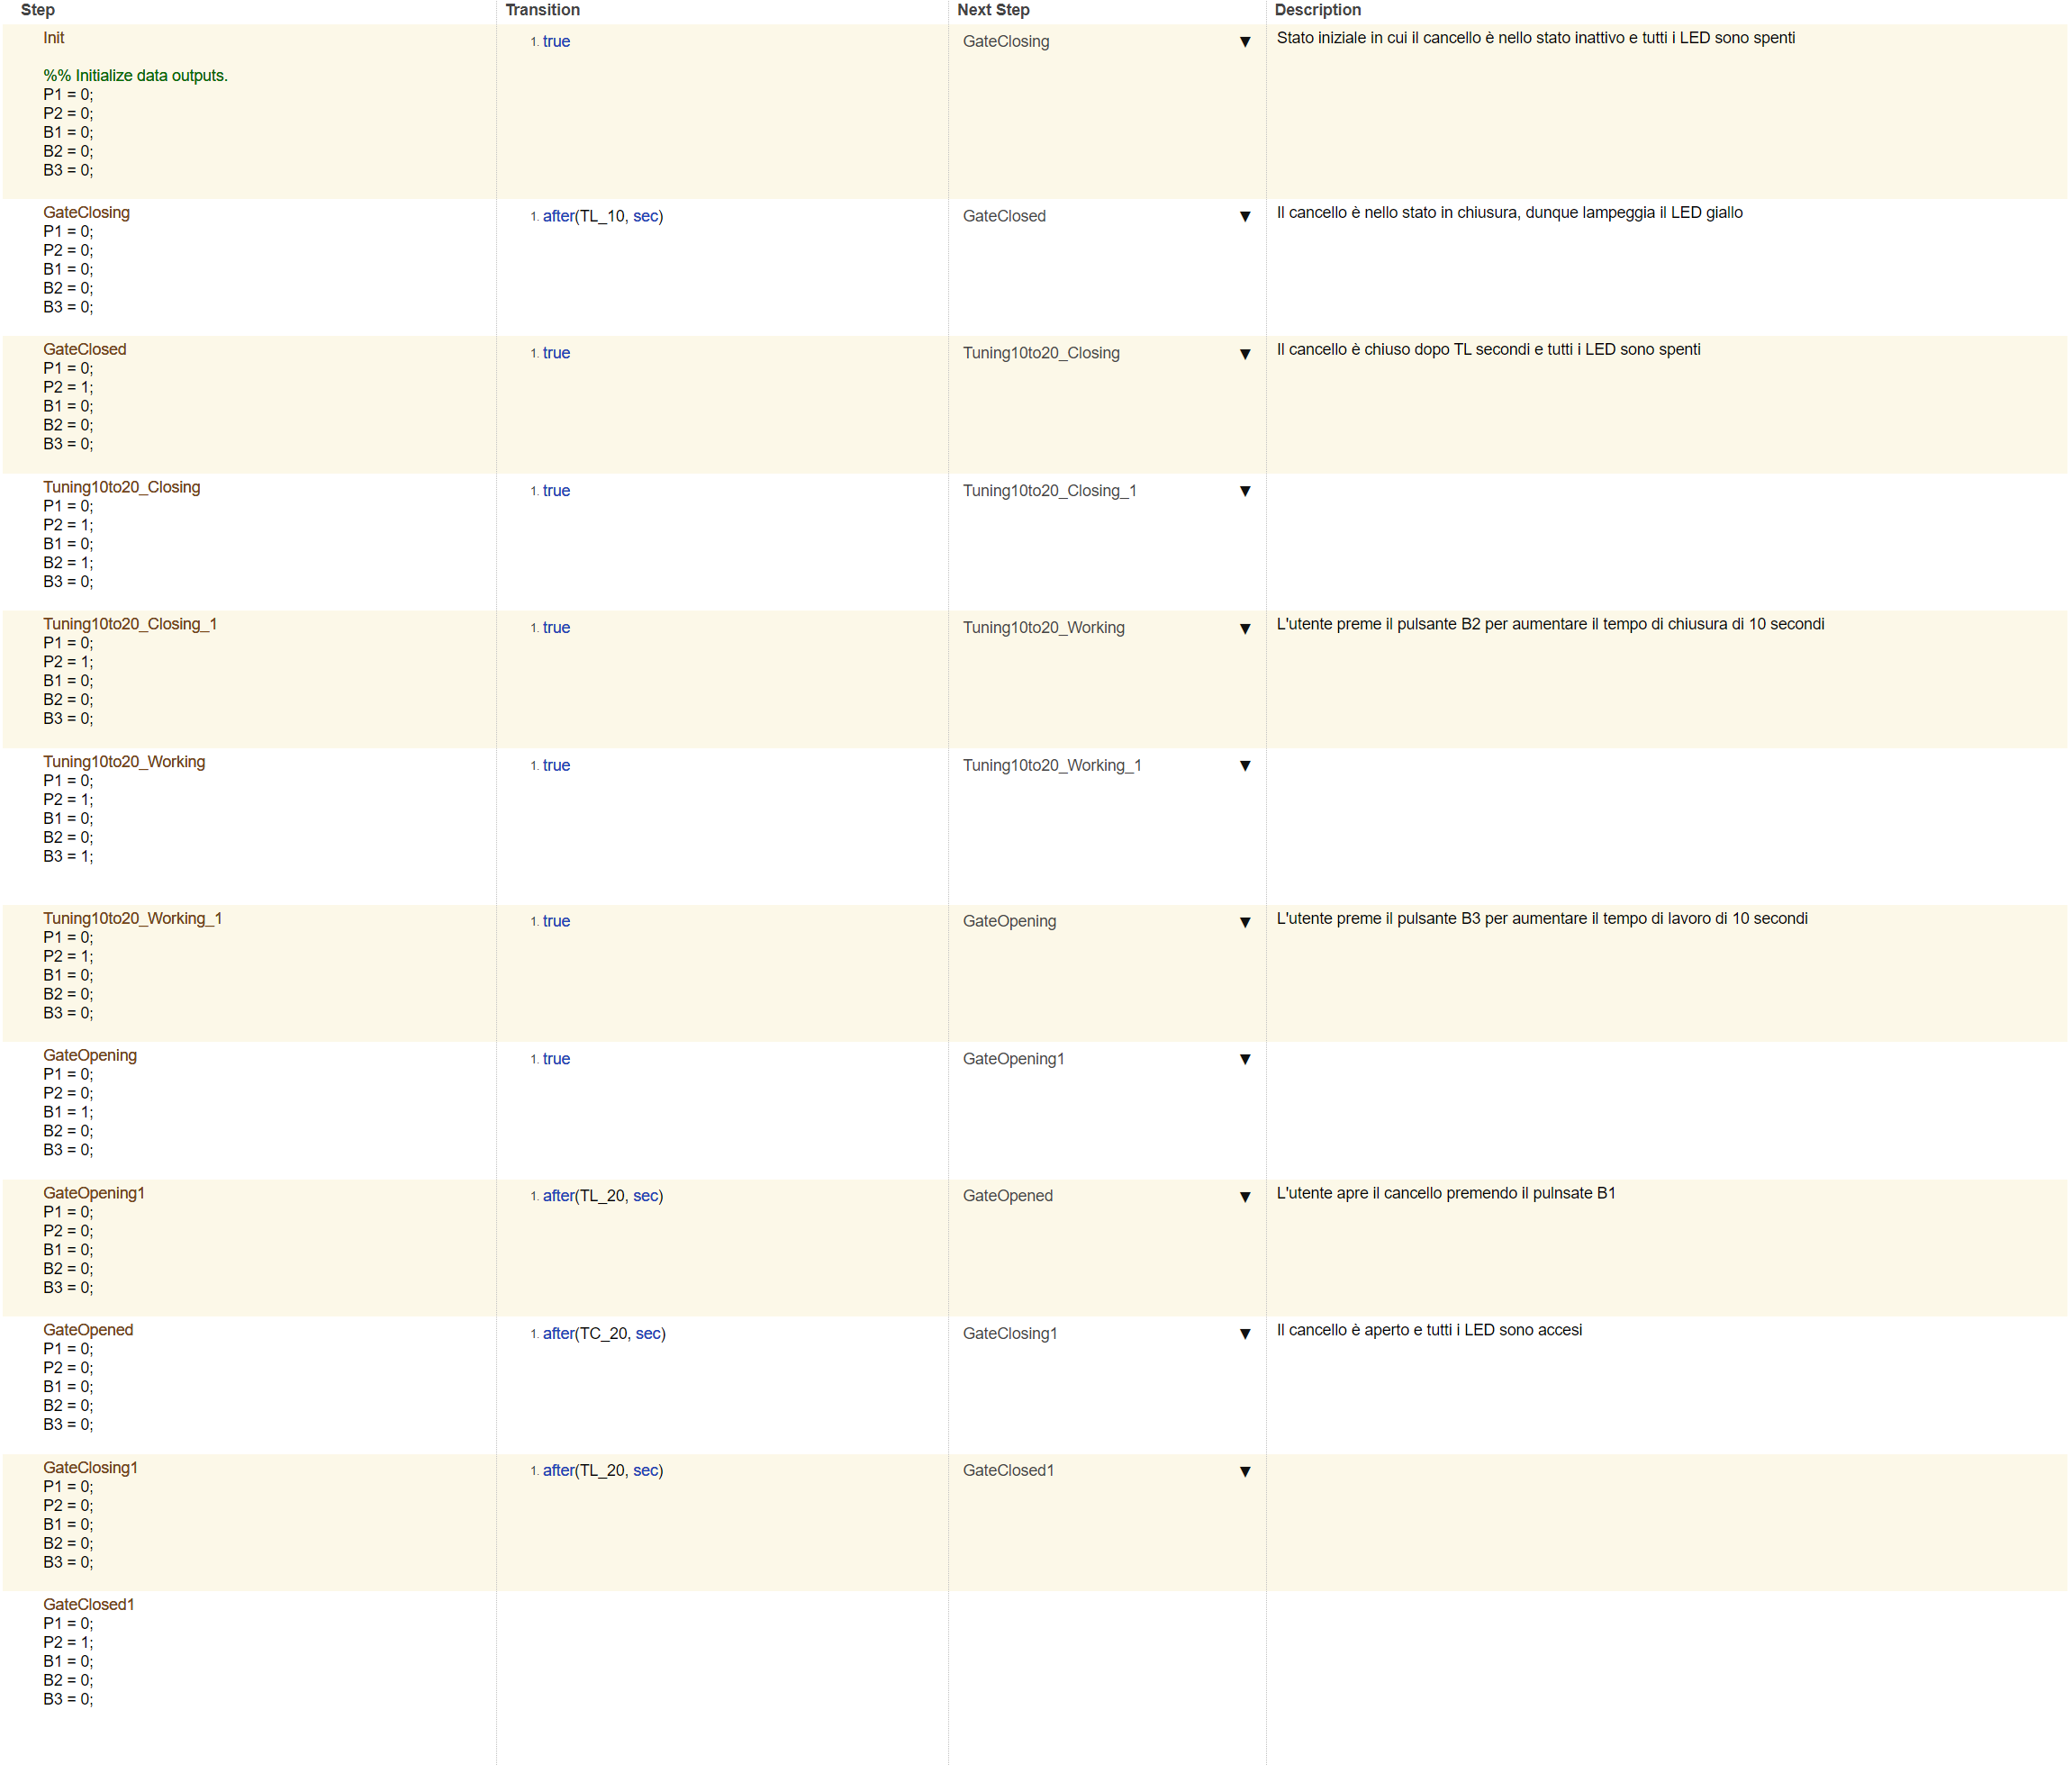
\includegraphics[width=0.9\textwidth]{figures/tuning_closing.png}
            \caption{Test Sequence}
            \label{tuningclos}
        \end{figure}

        \begin{figure}[H]
            \centering
            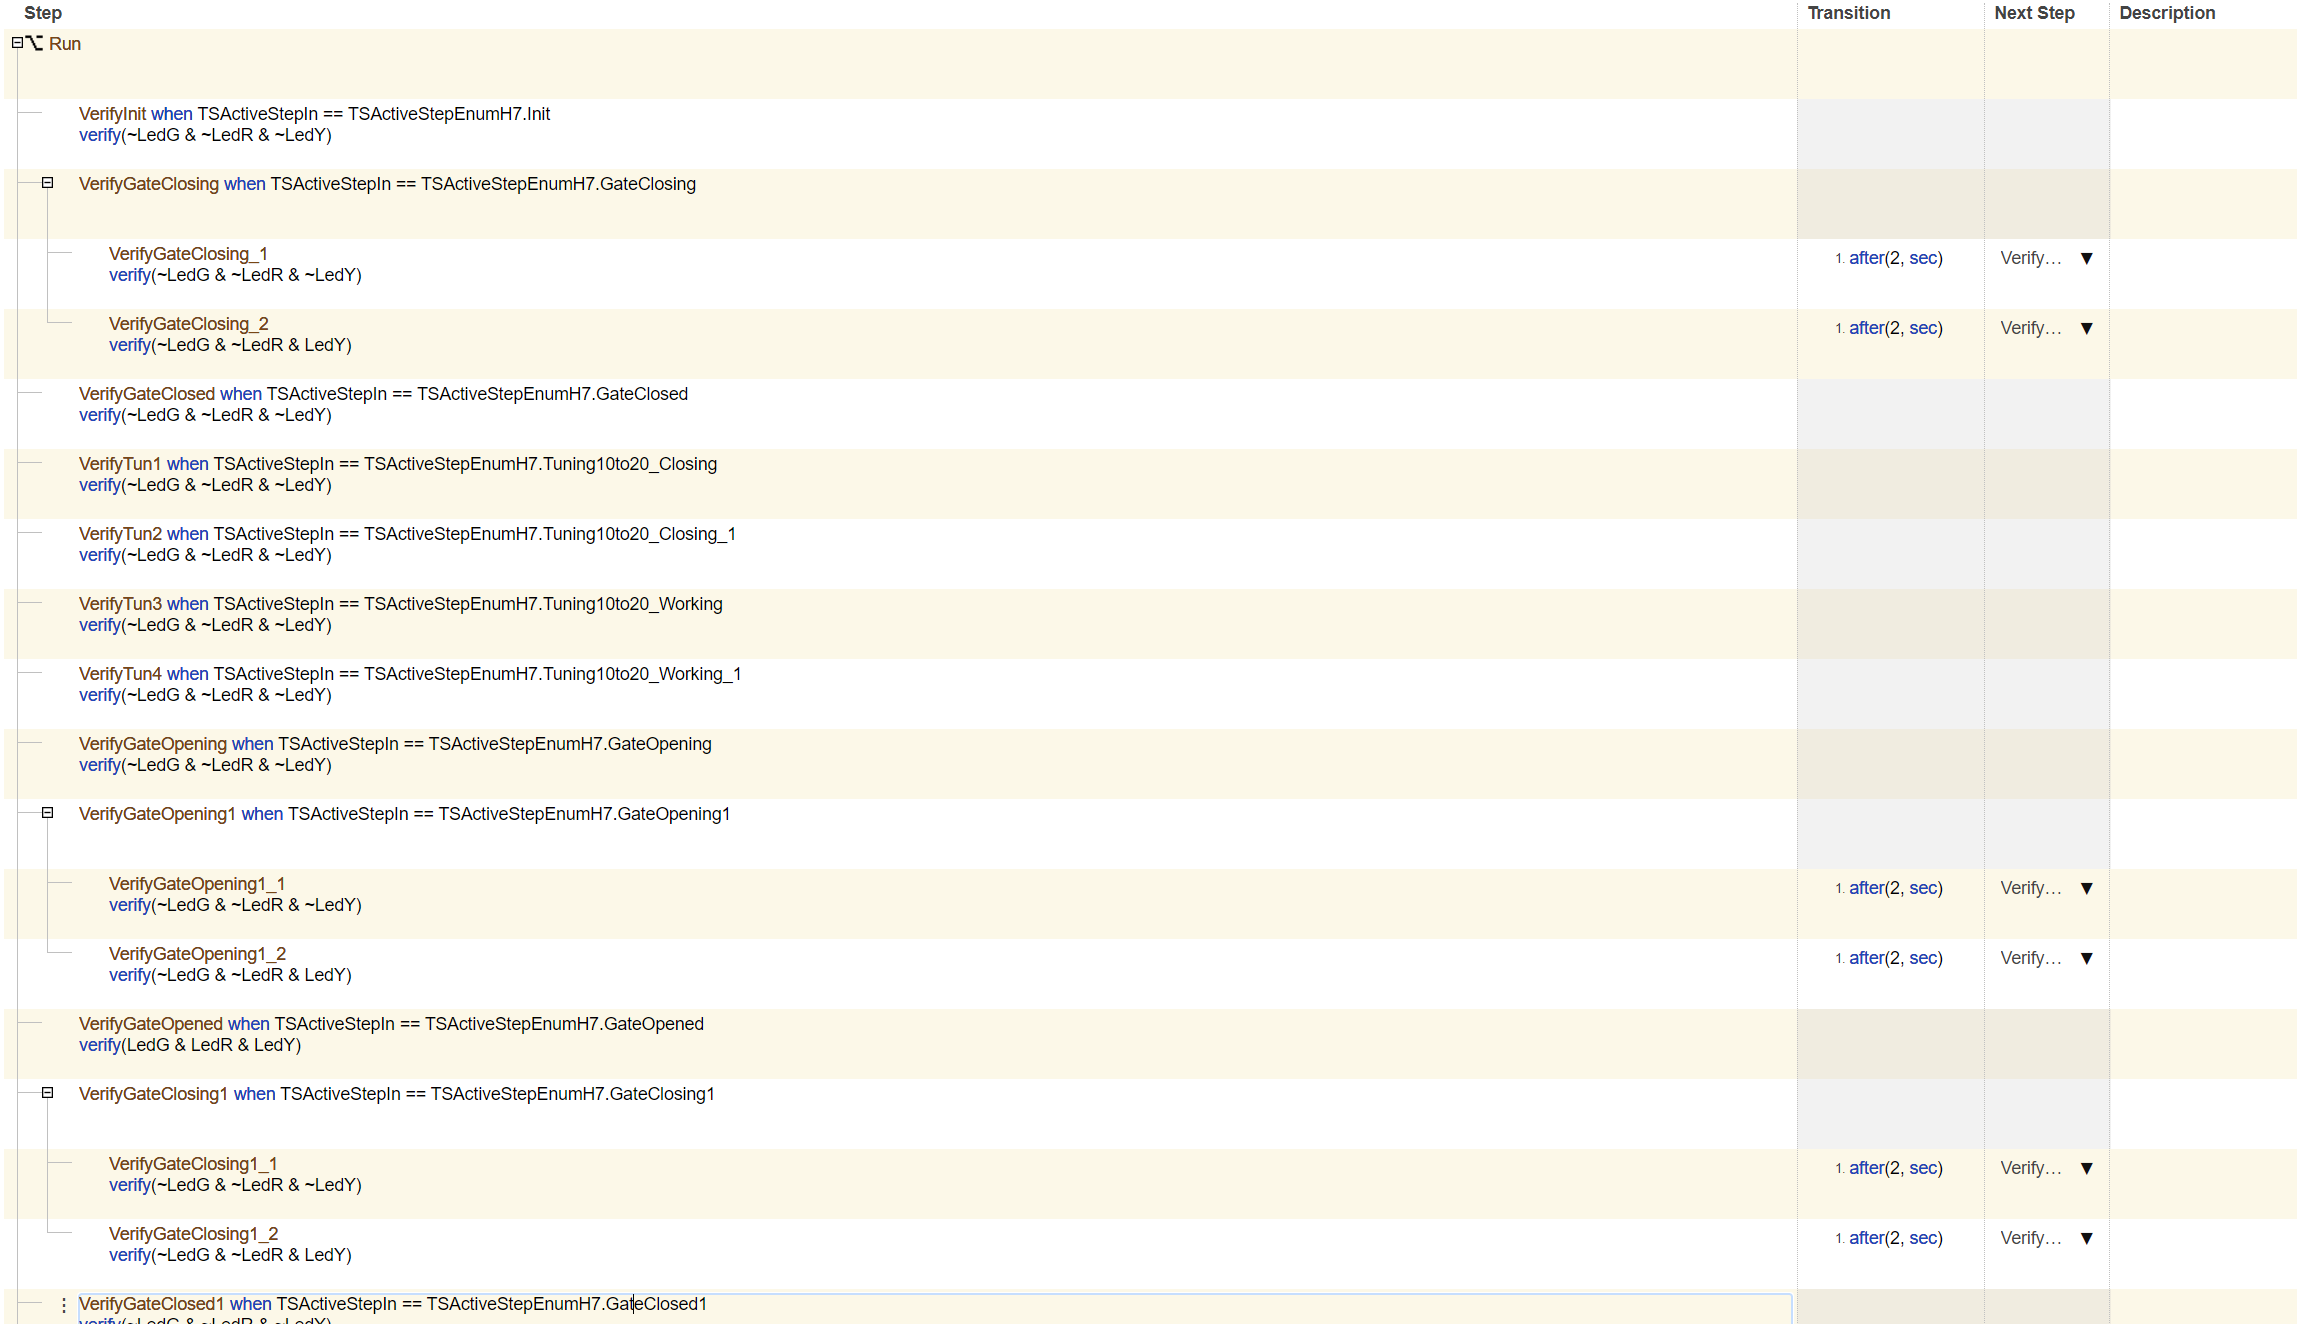
\includegraphics[width=0.9\textwidth]{figures/tuning_closing1.png}
            \caption{Test Assessment}
            \label{tuningclos1}
        \end{figure}


    \section{Regolazione $T_C$ e $T_L$ non nello stato Chiuso}
        Si riporta il test relativo al fallimento della regolazione del tempo di lavoro e del tempo di chiusura mentre il cancello non si trova nello stato \textbf{Chiuso}.
        In particolare, l'utente prova a regolare $T_C$ e $T_L$ premendo i pulsanti $B2$ e $B3$ mentre il cancello si trova nello stato \textbf{Aperto\_Con\_Ostacolo}, dunque la regolazione non avviene con successo e le due variabili precedentemente citate non cambiano il loro valore.

        \begin{figure}[H]
            \centering
            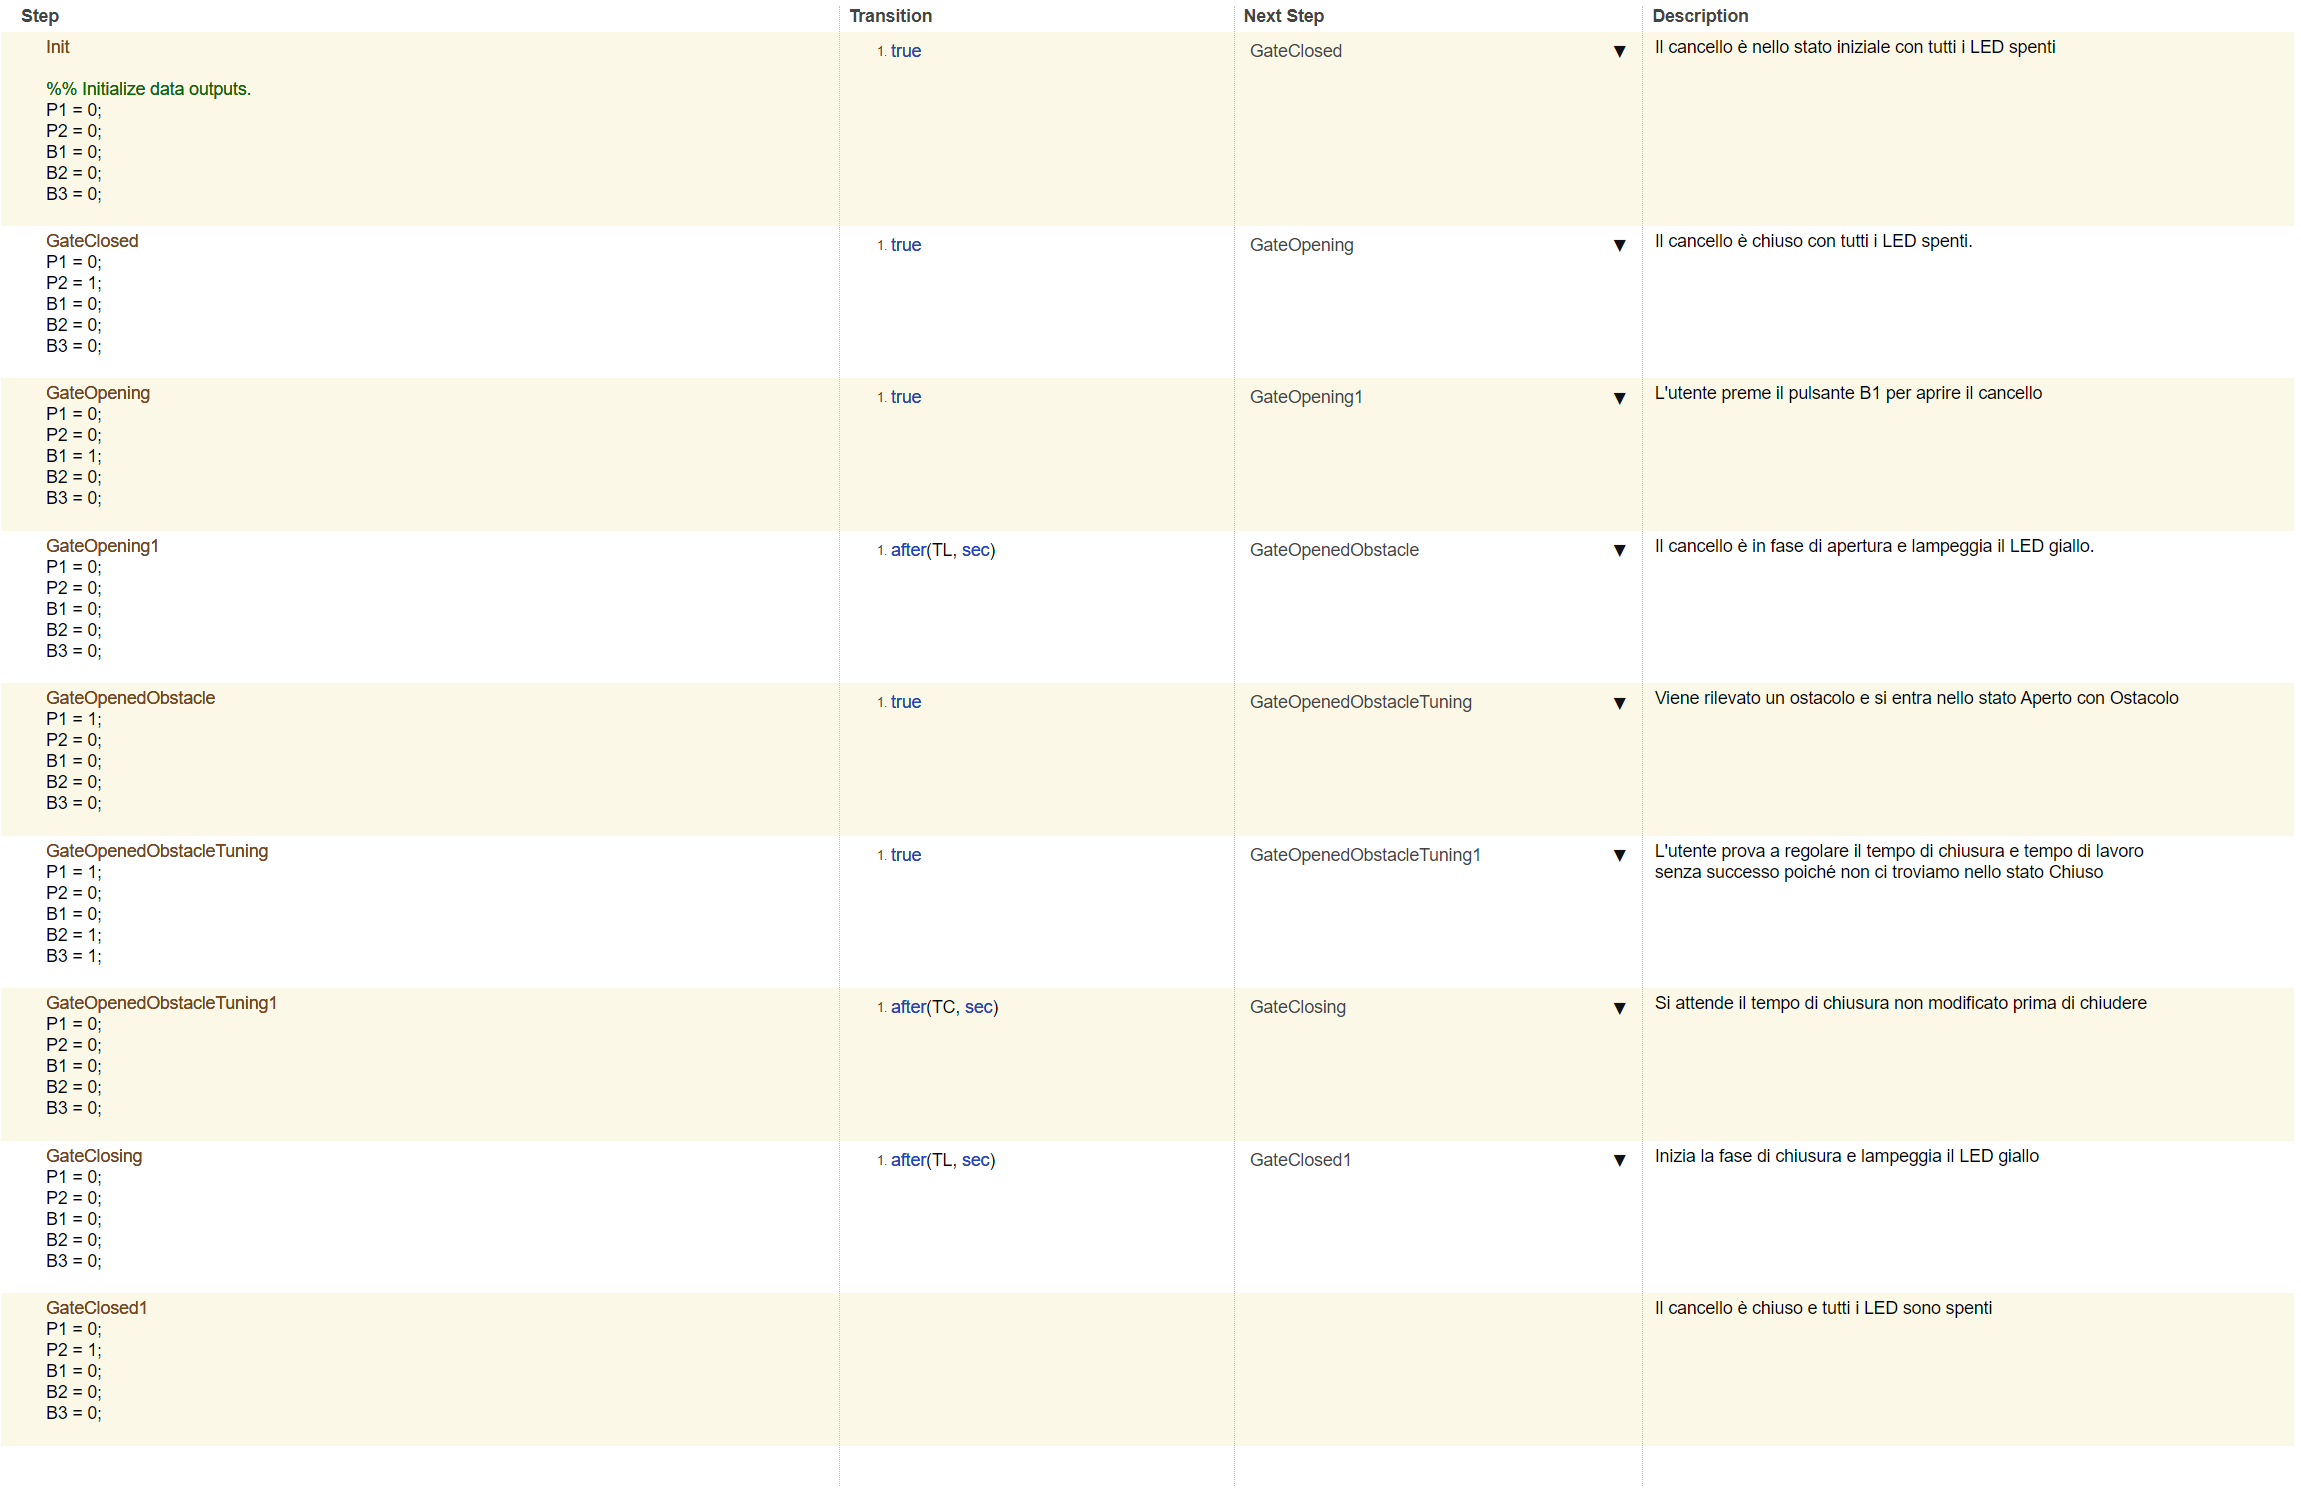
\includegraphics[width=0.9\textwidth]{figures/tuningOB.png}
            \caption{Test Sequence}
            \label{tuningob}
        \end{figure}
        
        \begin{figure}[H]
            \centering
            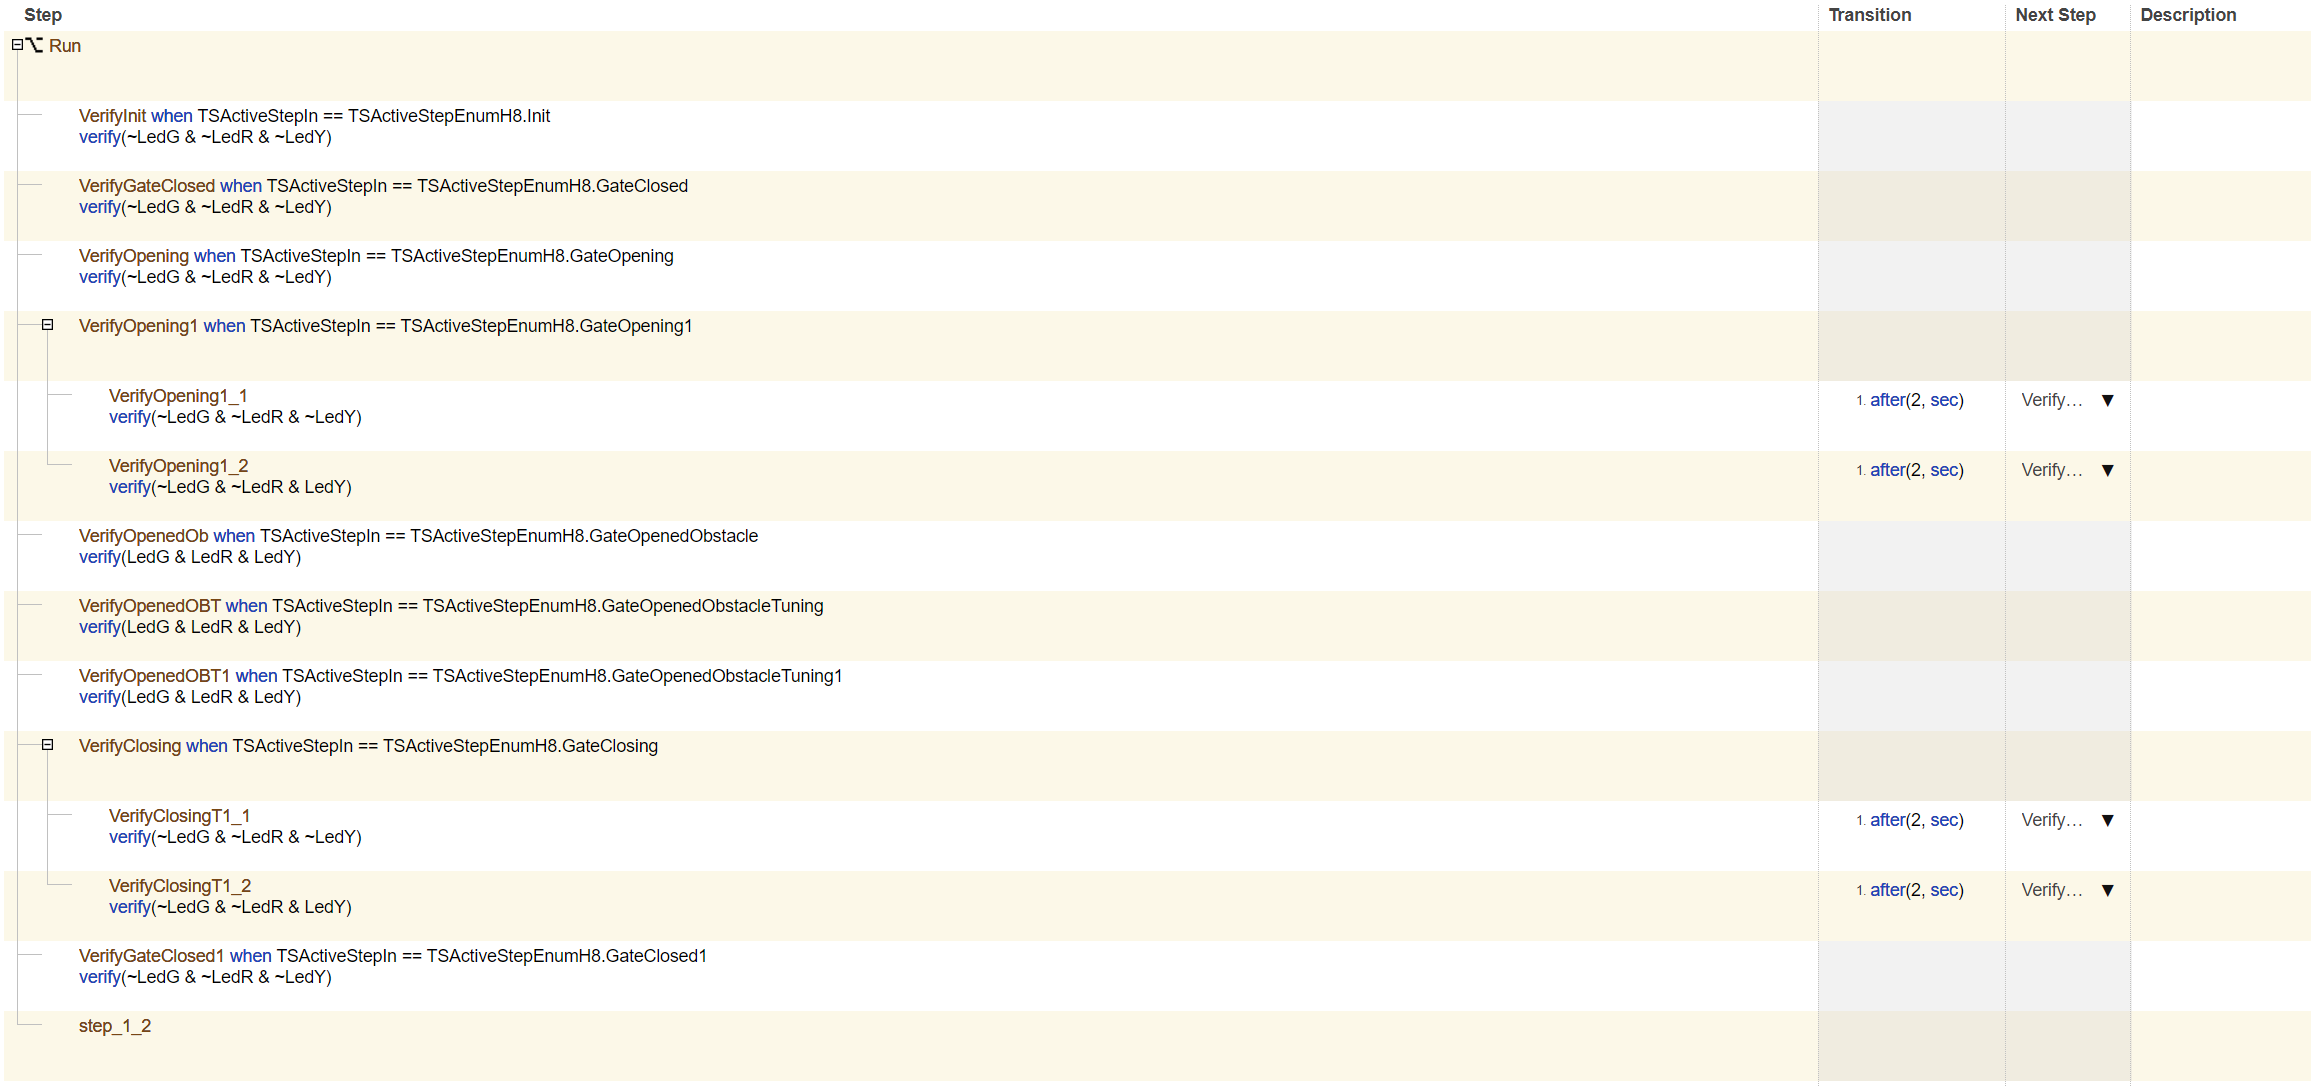
\includegraphics[width=0.9\textwidth]{figures/tuningOB1.png}
            \caption{Test Assessment}
            \label{tuningob1}
        \end{figure}


    \section{Reset del timer durante rilevazione Ostacolo}
    Si riporta il test relativo al reset del timer relativo al lampeggio del LED verde se l'utente preme ulteriormente il pulsante B1. In particolare, se ci si trova nello stato \textbf{Aperto\_Con\_Ostacolo}, se l'utente interagisce col pulsante B1 per chiudere il cancello, il LED verde inizia a lampeggiare per 30 secondi senza alcuna movimentazione del cancello. Il test dimostra che, qualora l'utente dovesse premere di nuovo il pulsante di chiusura (ad esempio dopo soli 5 secondi), il timer si resetta ed il conteggio riparte da 30 secondi.

    \begin{figure}[H]
            \centering
            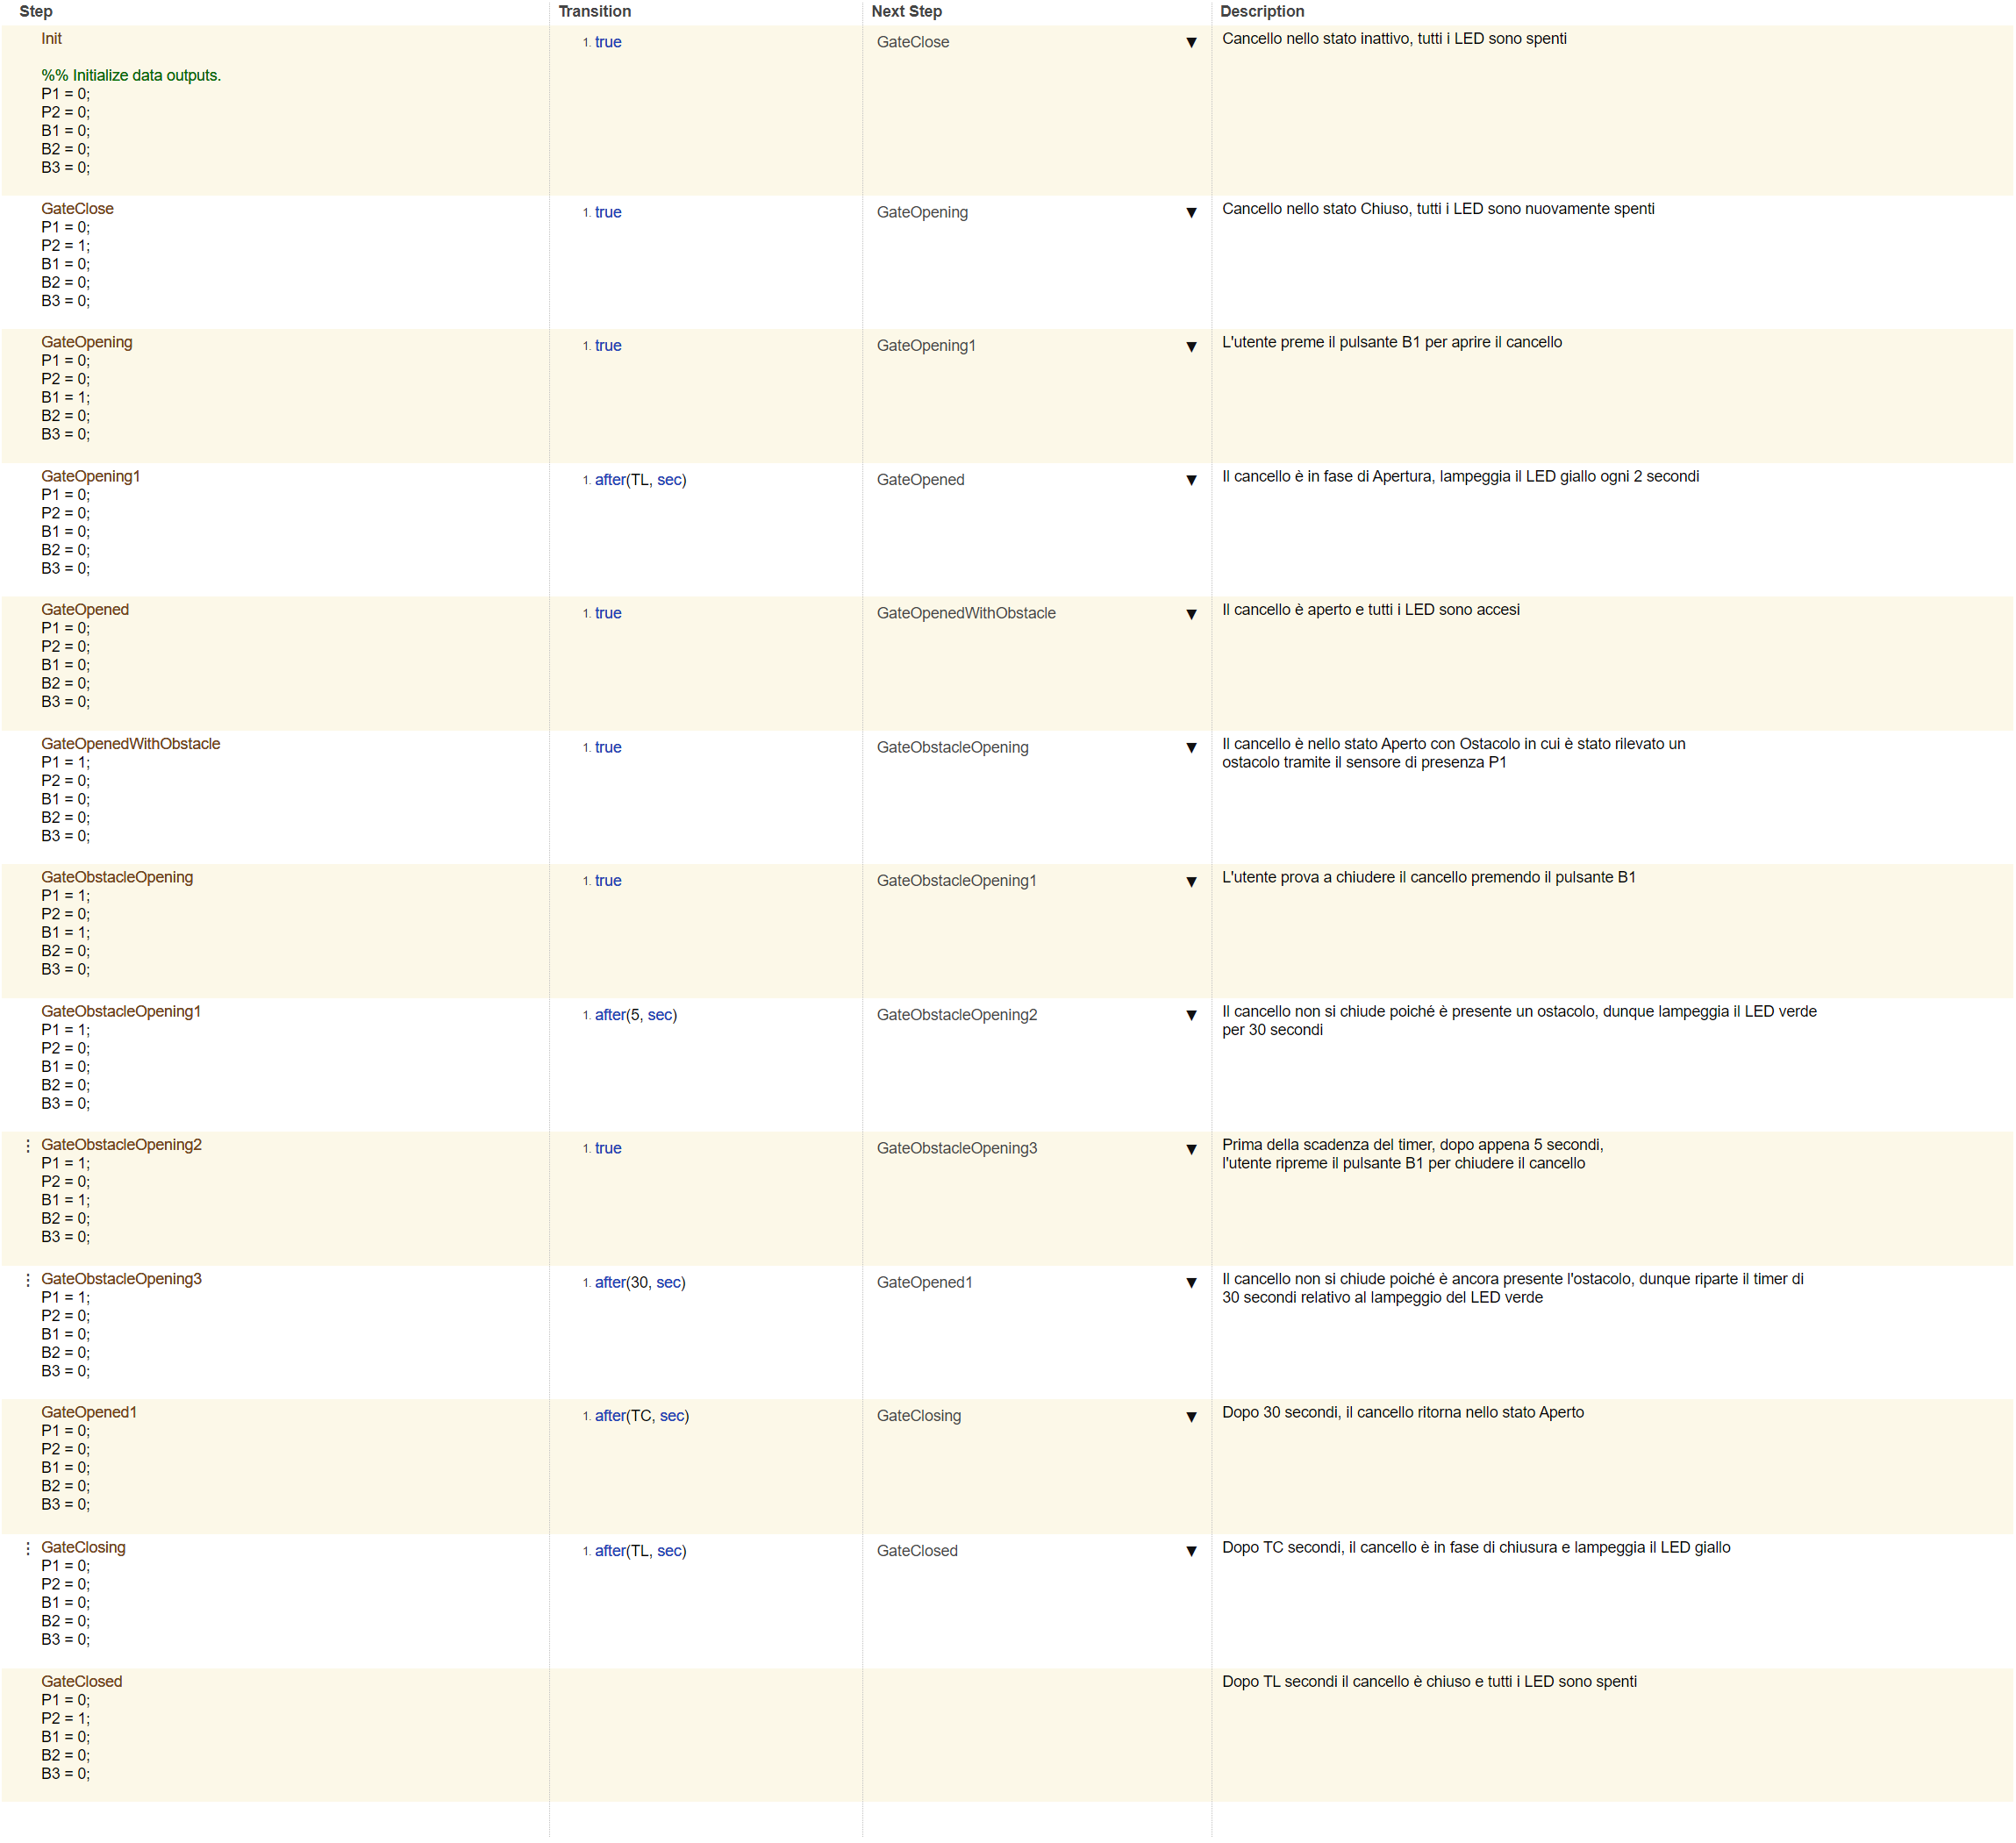
\includegraphics[width=0.9\textwidth]{figures/obstaclerepressed.png}
            \caption{Test Sequence}
            \label{obB1}
        \end{figure}
        
        \begin{figure}[H]
            \centering
            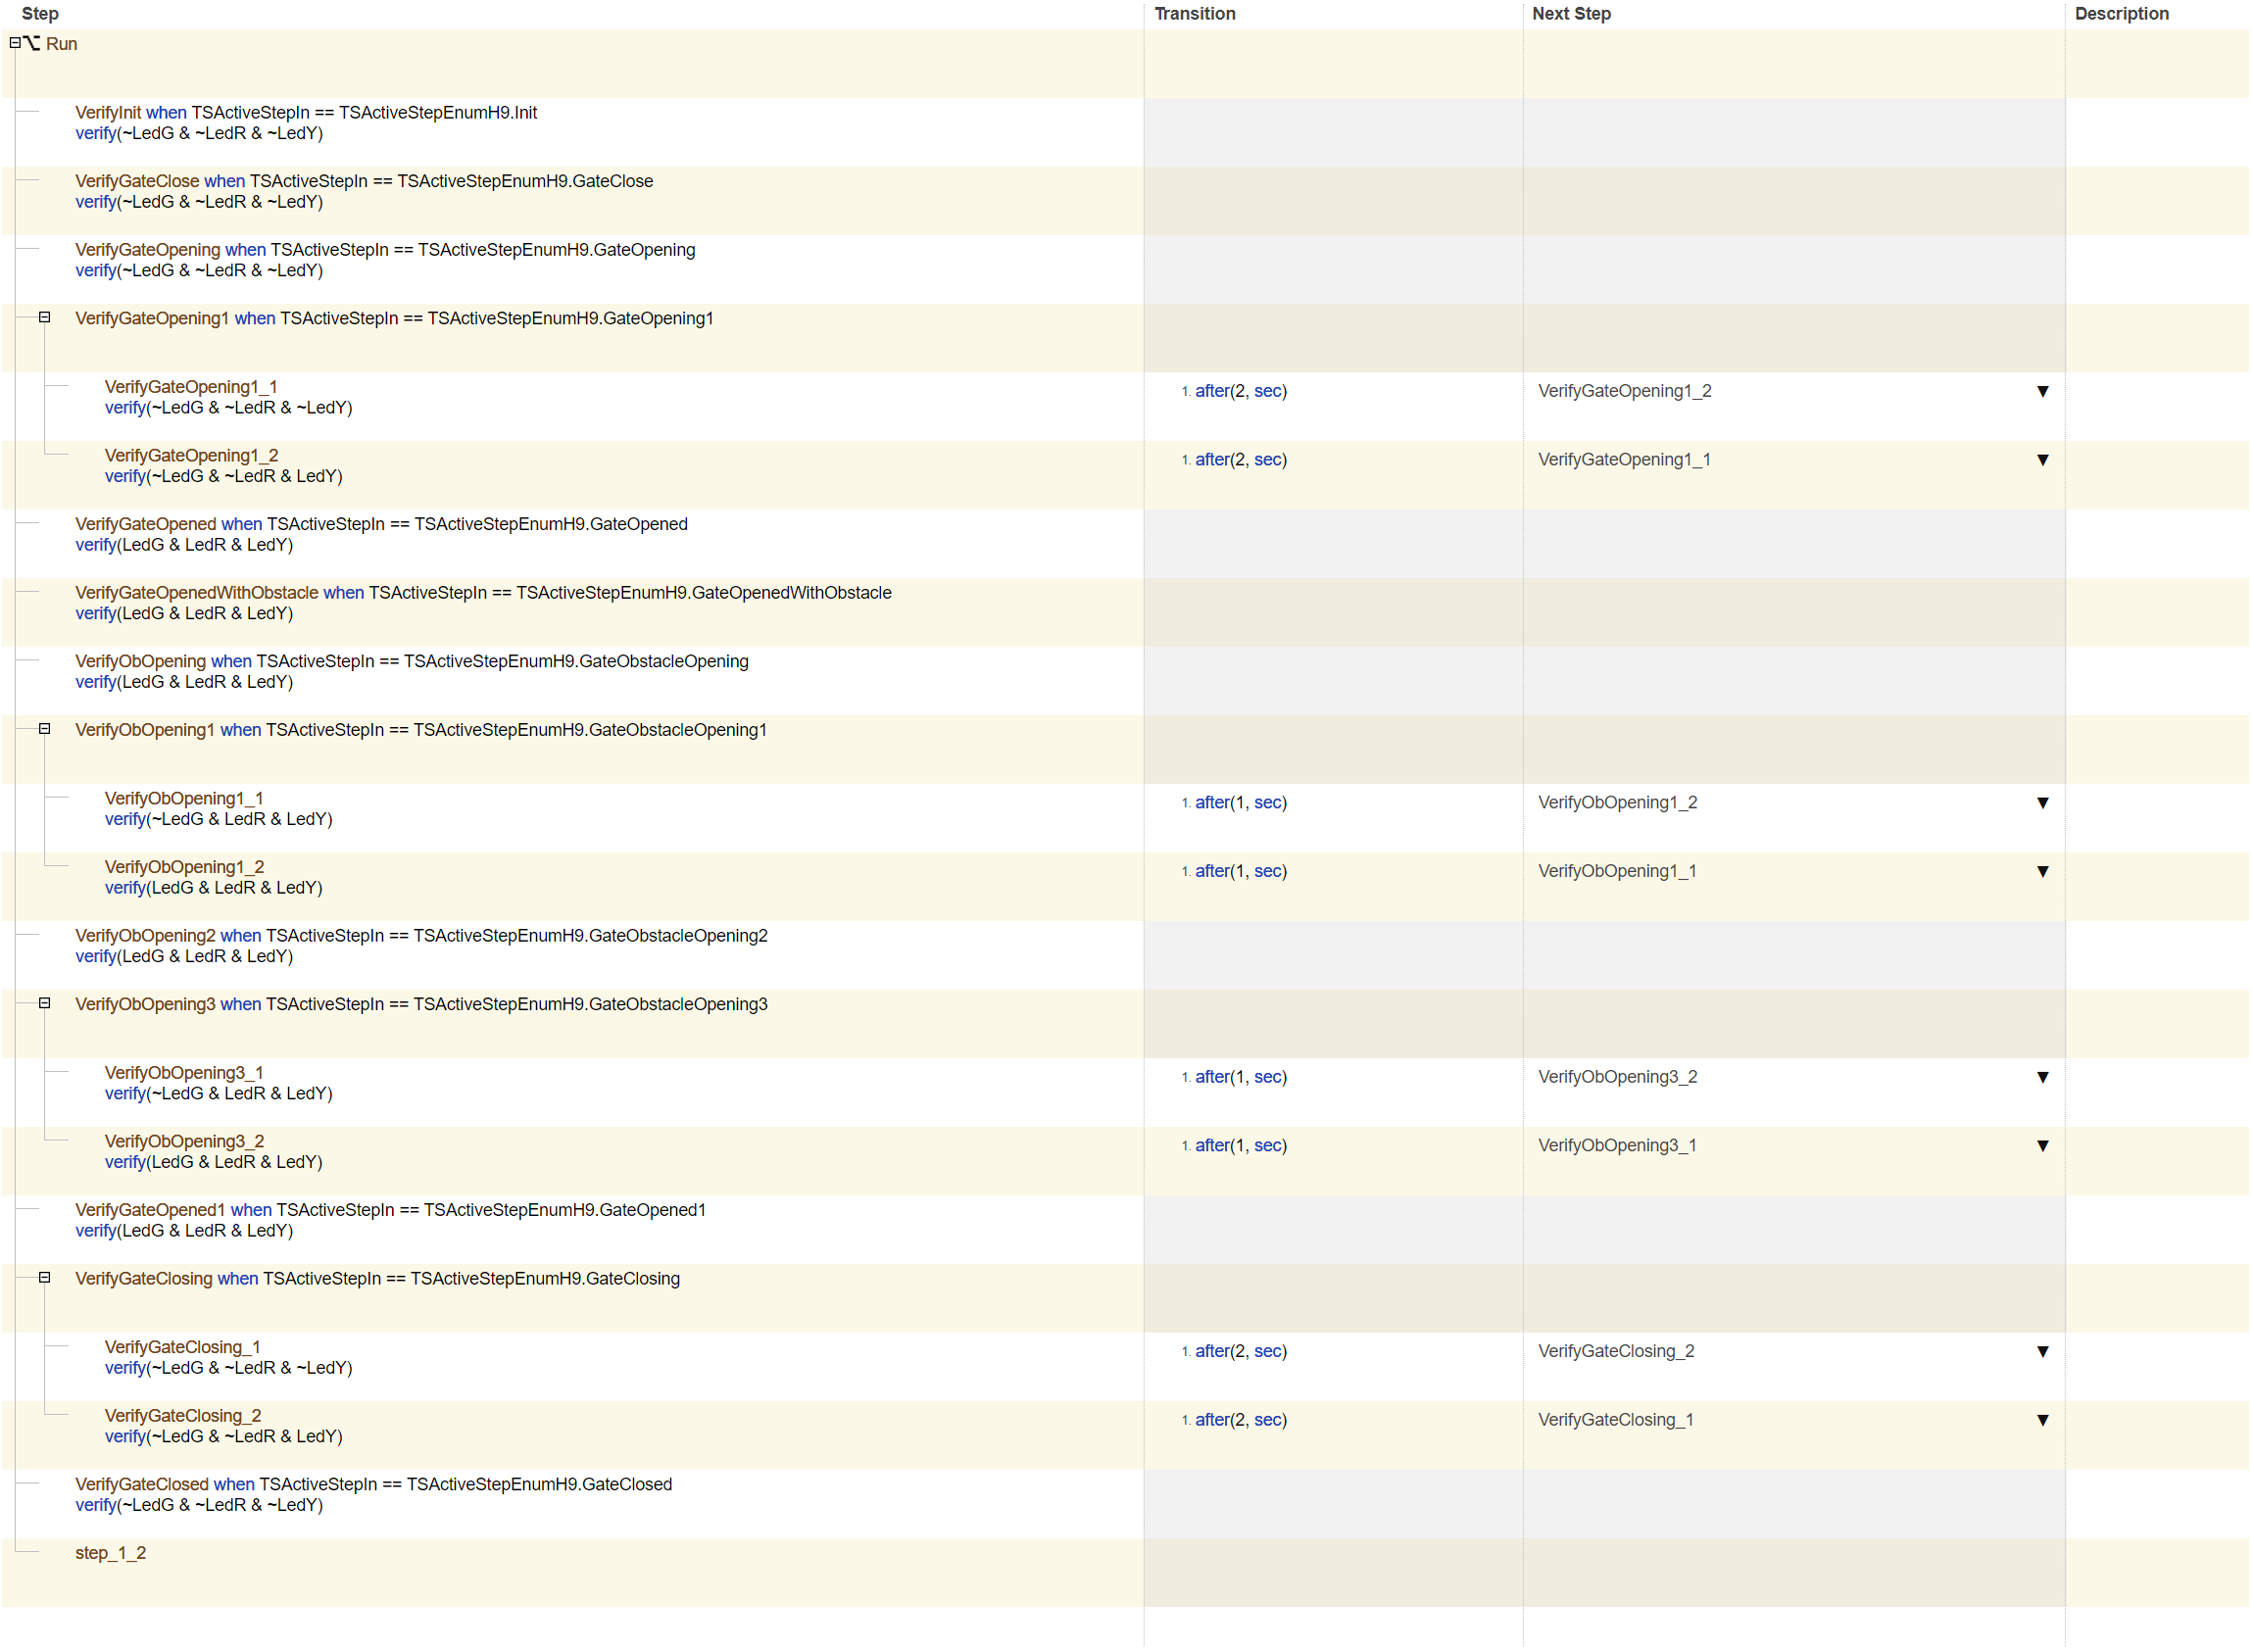
\includegraphics[width=0.9\textwidth]{figures/obstaclerepressed1.png}
            \caption{Test Assessment}
            \label{obB11}
        \end{figure}